% \documentclass[11pt,twoside]{book} %纸质版用twoside
\documentclass[12pt,oneside]{book} %电子版用oneside
\usepackage{setspace}

% \documentclass{article}

%%%%%%%%%%%%%%%%%%%%%%%%%%%%%%%%%%%%%%%%%%%%%%%%%%
%%%%%%%%%%%%%%%%%%%%% preamble %%%%%%%%%%%%%%%%%%%
%%%%%%%%%%%%%%%%%%%%%%%%%%%%%%%%%%%%%%%%%%%%%%%%%%

\usepackage[mono=false]{libertine} % new linux font, ignore mono

\usepackage{luatex85}

%\renewcommand{\baselinestretch}{1.05}
\usepackage{amsmath,amsthm,amssymb,mathrsfs,amsfonts,dsfont}
\usepackage{epsfig,graphicx}
\usepackage{tabularx}
\usepackage{blkarray}
\usepackage{slashed}
\usepackage{color}
\usepackage{listings}
\usepackage{caption}
% \usepackage{fullpage}
\usepackage{lipsum} % provides dummy text for testing
\usepackage[toc,title,titletoc,header]{appendix}
\usepackage{minitoc}
\usepackage{color}
\usepackage{multicol} % two-col ToC
\usepackage{bm}
\usepackage{imakeidx} % before hyperref
\usepackage{hyperref}
\usepackage{indentfirst}
\setlength{\parindent}{2em}


% link colors settings
\hypersetup{
    colorlinks=true,
    citecolor=magenta,
    linkcolor=blue,
    filecolor=green,      
    urlcolor=cyan,
    % hypertexnames=false,
}
\usepackage[capitalise]{cleveref}
\usepackage{subcaption}
\usepackage{enumitem}
\usepackage{mathtools}
\usepackage{physics}
\usepackage[linesnumbered,ruled,vlined,algosection]{algorithm2e}
\SetCommentSty{textsf}
\usepackage{epigraph}
\epigraphwidth=1.0\linewidth
\epigraphrule=0pt

% adjust margin
\usepackage[margin=2.3cm]{geometry}
\headheight13.6pt


\usepackage{graphicx}
\usepackage[justification=centering]{caption} % 图注居中
\usepackage{setspace}
\usepackage{geometry}
\usepackage{float}
\usepackage{hyperref}
\usepackage[utf8]{inputenc}
\usepackage[english]{babel}
\usepackage{framed}


\newcommand{\HRule}[1]{\rule{\linewidth}{#1}}





\setstretch{1.2}
% \geometry{
%     textheight=9in,
%     textwidth=5.5in,
%     top=1in,
%     headheight=12pt,
%     headsep=25pt,
%     footskip=30pt
% }





%%%%%%%%%%%%%%%% thmtools %%%%%%%%%%%%%%%%%%%%%

\usepackage{thmtools}
\usepackage[dvipsnames]{xcolor}
\usepackage[most]{tcolorbox}
\usepackage{enumerate}

\colorlet{LightGreen}{Green!15} %def
\colorlet{LightBlue}{Blue!15} %thm
\colorlet{LightOrange}{Orange!15} %lem
\colorlet{LightGray}{Gray!15}  %prop
\colorlet{LightRed}{Red!40} %cor
\colorlet{LightYellow}{Yellow!15} %exa


% \newtcbtheorem[
%   number within = chapter % 按每个 chapter 分别编号
% ]{definition% 环境名
% }{Definition% 这个参数可以设成“定理”“引理”“推论”等,编号就会变成“定理 1.1”“引理 1.1”“推论 1.1”等
% }{
%   attach title to upper = \par\vspace{1ex}, % 不要单独的标题栏,定理名完了之后分段,加上适量空白
%   separator sign = \quad, % 定理编号和定理名字之间用什么分隔;默认是冒号
%   sharp corners, % 直角;默认是圆角
%   enhanced jigsaw, frame hidden, % 隐藏 tcb 边框
%   colback = LightGreen, % 背景色
%   coltitle = blue!20!cyan!80!black, % 标题(定理编号和名字)的颜色
%   fonttitle = \sffamily\small, % 标题(定理编号和名字)的字体
%   description font = \normalsize, % 定理名字的字体
%   fontupper = \normalfont, % box 内的字体
% }{def% label 前缀
% }

\newtcbtheorem[
  auto counter,number within = chapter % 按每个 chapter 分别编号
]{definition% 环境名
}{Definition% 这个参数可以设成“定理”“引理”“推论”等,编号就会变成“定理 1.1”“引理 1.1”“推论 1.1”等
}{
  sharp corners, % 直角;默认是圆角
  colback=Green!5,
  colframe=Green!50!black,
  fonttitle=\sffamily\small
}{def% label 前缀
}


% 计数器设置
\makeatletter
\renewcommand\theHtcb@cnt@definition{\thechapter.\arabic{tcb@cnt@definition}}
\makeatother

\newtcbtheorem[
  auto counter,number within = chapter % 按每个 chapter 分别编号
]{theorem% 环境名
}{Theorem% 这个参数可以设成“定理”“引理”“推论”等,编号就会变成“定理 1.1”“引理 1.1”“推论 1.1”等
}{
  sharp corners, % 直角;默认是圆角
  colback=yellow!10,
  colframe=yellow!50!black,
  fonttitle=\sffamily\small
}{thm% label 前缀
}
% 计数器设置
\makeatletter
\renewcommand\theHtcb@cnt@theorem{\thechapter.\arabic{tcb@cnt@theorem}}
\makeatother

\newtcbtheorem[
  auto counter,number within = chapter % 按每个 chapter 分别编号
]{proposition% 环境名
}{Proposition% 这个参数可以设成“定理”“引理”“推论”等,编号就会变成“定理 1.1”“引理 1.1”“推论 1.1”等
}{
  sharp corners, % 直角;默认是圆角
  colback=Red!5,
  colframe=Red!50!black,
  fonttitle=\sffamily\small
}{prop% label 前缀
}
% 计数器设置
\makeatletter
\renewcommand\theHtcb@cnt@proposition{\thechapter.\arabic{tcb@cnt@proposition}}
\makeatother

\newtcbtheorem[
  auto counter,number within = chapter % 按每个 chapter 分别编号
]{corollary% 环境名
}{Corollary% 这个参数可以设成“定理”“引理”“推论”等,编号就会变成“定理 1.1”“引理 1.1”“推论 1.1”等
}{
  sharp corners, % 直角;默认是圆角
  colback=Blue!5,
  colframe=Blue!50!black,
  fonttitle=\sffamily\small
}{cor% label 前缀
}

% 计数器设置
\makeatletter
\renewcommand\theHtcb@cnt@corollary{\thechapter.\arabic{tcb@cnt@corollary}}
\makeatother

\newtcbtheorem[
  auto counter,number within = chapter % 按每个 chapter 分别编号
]{lemma% 环境名
}{Lemma% 这个参数可以设成“定理”“引理”“推论”等,编号就会变成“定理 1.1”“引理 1.1”“推论 1.1”等
}{
  sharp corners, % 直角;默认是圆角
  colback=Gray!10,
  colframe=Gray!50!black,
  fonttitle=\sffamily\small
}{lem% label 前缀
}

% 计数器设置
\makeatletter
\renewcommand\theHtcb@cnt@lemma{\thechapter.\arabic{tcb@cnt@lemma}}
\makeatother


\newtcbtheorem[
  auto counter,number within = chapter % 按每个 chapter 分别编号
]{example}
{Example}%
  {
    enhanced, breakable,
    colback = white, colframe = purple, colbacktitle = purple,
    attach boxed title to top left = {yshift = -2mm, xshift = 5mm},
    boxed title style = {sharp corners},
    fonttitle=\sffamily\small
  }
{exa}

% 计数器设置
\makeatletter
\renewcommand\theHtcb@cnt@example{\thechapter.\arabic{tcb@cnt@example}}
\makeatother


\newtcbtheorem[
  auto counter,number within = chapter % 按每个 chapter 分别编号
]{exercise}
{Exercise}%
  {
    enhanced, breakable,
    colback = white, colframe = cyan, colbacktitle = cyan,
    attach boxed title to top left = {yshift = -2mm, xshift = 5mm},
    boxed title style = {sharp corners},
    fonttitle=\sffamily\small
  }
{exer}

% 计数器设置
\makeatletter
\renewcommand\theHtcb@cnt@exercise{\thechapter.\arabic{tcb@cnt@exercise}}
\makeatother


% \declaretheorem[numberwithin=chapter,shaded={rulecolor=LightGreen,
% rulewidth=2pt,bgcolor=LightGreen,
% textwidth=12em}]{definition}

\usepackage{changepage}
\newenvironment{remark}{\underline{\textbf{Remark.}}}{\par}

\newenvironment{proofsolution}
    {\renewcommand\qedsymbol{$\square$}\color{blue}\begin{adjustwidth}{0em}{2em}\begin{proof}[\textit Proof.~]}
    {\end{proof}\end{adjustwidth}}


%%%%%%%%%%%%%%%% index %%%%%%%%%%%%%%%%%%%%%
\begin{filecontents}{index.ist}
% https://tex.stackexchange.com/questions/65247/index-with-an-initial-letter-of-the-group
headings_flag 1
heading_prefix "{\\centering\\large \\textbf{"
heading_suffix "}}\\nopagebreak\n"
delim_0 "\\nobreak\\dotfill"
\end{filecontents}
\newcommand{\myindex}[1]{\index{#1} \emph{#1}}
\makeindex[columns=3, intoc, title=Alphabetical Index, options= -s index.ist]
%%%%%%%%%%%%%%%% index %%%%%%%%%%%%%%%%%%%%%

%%%%%%%%%%%%%%%% ToC %%%%%%%%%%%%%%%%%%%%%
% Link Chapter title to ToC: https://tex.stackexchange.com/questions/32495/linking-the-section-text-to-the-toc
\usepackage[explicit]{titlesec}
\titleformat{\chapter}[display]
  {\normalfont\huge\bfseries}{\chaptertitlename\ {\thechapter}}{20pt}{\hyperlink{chap-\thechapter}{\Huge#1}
\addtocontents{toc}{\protect\hypertarget{chap-\thechapter}{}}}
\titleformat{name=\chapter,numberless}
  {\normalfont\huge\bfseries}{}{-20pt}{\Huge#1}

%%%%%%%%%%%%%%%%%%% fancyhdr %%%%%%%%%%%%%%%%%
\usepackage{fancyhdr}
\pagestyle{fancy} % enable fancy page style
\renewcommand{\headrulewidth}{0.0pt} % comment if you want the rule
\fancyhf{} % clear header and footer
\fancyhead[lo,le]{\leftmark}
\fancyhead[re,ro]{\rightmark}
\fancyfoot[CE,CO]{\hyperref[toc-contents]{\thepage}}

% https://tex.stackexchange.com/questions/550520/making-each-page-number-link-back-to-beginning-of-chapter-or-section
\makeatletter
\def\chaptermark#1{\markboth{\protect\hyper@linkstart{link}{\@currentHref}{Chapter \thechapter ~ #1}\protect\hyper@linkend}{}}
\def\sectionmark#1{\markright{\protect\hyper@linkstart{link}{\@currentHref}{\thesection ~ #1}\protect\hyper@linkend}}
\makeatother
%%%%%%%%%%%%%%%%%%% fancyhdr %%%%%%%%%%%%%%%%%


%%%%%%%%%%%%%%%%%%% biblatex %%%%%%%%%%%%%%%%%
\usepackage[doi=false,url=false,isbn=false,style=alphabetic,backend=biber,backref=true]{biblatex}
\addbibresource{bib.bib}

\newbibmacro{string+doiurlisbn}[1]{%
  \iffieldundef{doi}{%
    \iffieldundef{url}{%
      \iffieldundef{isbn}{%
        \iffieldundef{issn}{%
          #1%
        }{%
          \href{http://books.google.com/books?vid=ISSN\thefield{issn}}{#1}%
        }%
      }{%
        \href{http://books.google.com/books?vid=ISBN\thefield{isbn}}{#1}%
      }%
    }{%
      \href{\thefield{url}}{#1}%
    }%
  }{%
    \href{http://dx.doi.org/\thefield{doi}}{#1}%
  }%
}

% https://tex.stackexchange.com/questions/94089/remove-quotes-from-inbook-reference-title-with-biblatex
\DeclareFieldFormat[article,incollection,inproceedings,book,misc]{title}{\usebibmacro{string+doiurlisbn}{\mkbibemph{#1}}}
% https://tex.stackexchange.com/questions/454672/biblatex-journal-name-non-italic
\DeclareFieldFormat{journaltitle}{#1\isdot}
\DeclareFieldFormat{booktitle}{#1\isdot}
% https://tex.stackexchange.com/questions/10682/suppress-in-biblatex
\renewbibmacro{in:}{}
% add video field: https://tex.stackexchange.com/questions/111846/biblatex-2-custom-fields-only-one-is-working
\DeclareSourcemap{
    \maps[datatype=bibtex]{
      \map{
        \step[fieldsource=video]
        \step[fieldset=usera,origfieldval]
    }
  }
}
\DeclareFieldFormat{usera}{\href{#1}{\textsc{Online video}}}
\AtEveryBibitem{
    \csappto{blx@bbx@\thefield{entrytype}}{% put at end of entry
        \iffieldundef{usera}{}{\space \printfield{usera}}
    }
}


%%%%%%%%%%%%%%%%%%%%%%%notations%%%%%%%%%%%%%%%%%%%%%%%%%%%%%%
\newcommand{\F}{\ensuremath{\mathbb{F}}}
\newcommand{\C}{\ensuremath{\mathbb{C}}} 
\newcommand{\R}{\ensuremath{\mathbb{R}}}
\newcommand{\J}{\ensuremath{\mathbb{J}}}
\newcommand{\Q}{\ensuremath{\mathbb{Q}}}
\newcommand{\Z}{\ensuremath{\mathbb{Z}}}
\newcommand{\N}{\ensuremath{\mathbb{N}}}
\newcommand{\K}{\ensuremath{\mathbb{K}}}
\newcommand{\Zo}{\ensuremath{\mathbb{Z}_{\geqslant 0}}} % 非负整数集
\newcommand{\Zi}{\ensuremath{\mathbb{Z}_{\geqslant 1}}} % 正整数集
\newcommand{\id}{\mathrm{id}}
\newcommand{\im}{\mathrm{im}\,}                         % 映射的像
\newcommand{\leqs}{\leqslant}
\newcommand{\geqs}{\geqslant}
\newcommand{\ci}{\mathrm{i}}
\newcommand{\hH}{\mathscr{H}}
\newcommand{\hK}{\mathscr{K}}
\newcommand{\inner}[2]{\langle#1,#2\rangle}

%%%%%%%%%%%%%%%%%%% biblatex %%%%%%%%%%%%%%%%%

%%%%%%%%%%%%%%%%%%%%% glossaries %%%%%%%%%%%%%%%%%
% !TEX root = ./notes_template.tex
% \usepackage[style=super]{glossaries}
% https://www.overleaf.com/learn/latex/Glossaries
\usepackage[style=super,toc,acronym]{glossaries}
\setlength{\glsdescwidth}{1\linewidth}
\makeglossaries

\renewcommand\glossaryname{List of Abbreviations and Symbols}

\newglossaryentry{Q2}{name={$Q_2(f)$},
%sort=Q2,
description={Two-side (bounded) error quantum query complexity}}

\newglossaryentry{real_number}{name={$\mathbb{R}$},description={Real number}}

% \newglossaryentry{gcd}{name={gcd},description={greatest common divisor}}

\newacronym{gcd}{GCD}{Greatest Common Divisor}


\newglossaryentry{svm}{name={SVM},description={Support Vector Machine}}

\newglossaryentry{gd}{name={GD},description={Gradient Descent}}

\newglossaryentry{qft}{name={QFT},description={Quantum Field Theory}}

\newglossaryentry{qm}{name={QM},description={Quantum Mechanics}}

\newglossaryentry{v}{name={$\vec{v}$},description={a vector}}

% physics
\newglossaryentry{hamiltonian}{name={$\hat{H}$},description={Hamiltonian}}

\newglossaryentry{lagrangian}{name={$L$},description={Lagrangian}}
%%%%%%%%%%%%%%%%%%%%% glossaries %%%%%%%%%%%%%%%%%

%%%%%%%%%%%%%%%%%%%%% glossaries-extra %%%%%%%%%%%%%%%%%
% \usepackage[record,abbreviations,symbols,stylemods={list,tree,mcols}]{glossaries-extra}
%%%%%%%%%%%%%%%%%%%%% glossaries-extra %%%%%%%%%%%%%%%%%


% !TEX root = ./notes_template.tex

%%%%%%%%%%%%%%%%%%%%%%%%%%%%%%%%%%%%
%%%%%%%%%%%%%%%%%%%%%%%%%%%%%%%%%%%%
% math
\let\iff\relax
\newcommand{\iff}{\text{ iff }}
\newcommand{\OPT}{\textup{OPT}}

% physics
\newcommand{\acreation}{a^\dagger}



%%%%%%%%%%%%%%%%%%%%%%%%%%%%%%%%%%%%%%%%%%%%%%%%%%
%%%%%%%%%%%%%%%% begin of document %%%%%%%%%%%%%%%
%%%%%%%%%%%%%%%%%%%%%%%%%%%%%%%%%%%%%%%%%%%%%%%%%%

\begin{document}

\title{\bf \huge Study Notes of Topology}
\author{Pei Zhong}
\date{Update on \today}

\maketitle

% \newpage
% \let\cleardoublepag\clearpage

\tableofcontents

\begin{spacing}{1}

%%%%%%%%%%%%%%update progress%%%%%%%%%%



%%%%%%%%%%%%%%update progress end%%%%%%%%




%%%%%%%%%%%%%%%preface%%%%%%%%%%%%%

\chapter*{Preface}

Notes mainly refer to following materials:


\begin{itemize}
    \item[*] Machine learning
    \begin{itemize}
        \item \href{https://www.cs.cornell.edu/courses/cs4780/2023sp/}{lecture notes from cornell}
        \item \href{https://www.cs.cmu.edu/~hn1/documents/machine-learning/notes.pdf}{lecture notes from cmu}
        \item \href{https://cs229.stanford.edu/main_notes.pdf}{lecture notes of CS229}
    \end{itemize}
    \item[*] Deep learning
    \begin{itemize}
        \item \href{https://udlbook.github.io/udlbook/}{understanding deep learning}
        \item \href{https://www.bilibili.com/video/BV1Wv411h7kN/?spm_id_from=333.337.search-card.all.click}{lecture video from Hongyi Lee}
        \item \href{https://cs231n.github.io/}{lecture notes from Stanford}
    \end{itemize}
    \item[*] Reinforcement learning
    \begin{itemize}
        \item \href{https://web.stanford.edu/class/cs234/modules.html}{lecture notes from stanford}
        \item \href{https://people.cs.umass.edu/~bsilva/courses/CMPSCI_687/Fall2022/Lecture_Notes_v1.0_687_F22.pdf}{lecture notes from umass}
    \end{itemize}
\end{itemize}







\chapter{Preliminary Knowledge}\label{chp:0_1}

\section{Countability}




\section{Reference}
\begin{itemize}
    \item Countability: \href{https://www.math.toronto.edu/ivan/mat327/docs/notes/04-countability.pdf}{lecture notes from toronto}
\end{itemize}
%%%%%%%%%%%%%preface end%%%%%%%%%%%%%

\part{Topology Space and Continuity}
\chapter{Topological Space}\label{1_1}

This chapter opens with the definition of a topology and 
is then devoted to some simple examples.
\par
Topology, like other branches of pure mathematics such group theory,
is an axiomatic subjece. We start with a set of axioms and we use these 
axioms and we use these axioms to prove propositions and theorems. 
It is extremely important to develop your skill at writing proofs.
\section{Topological Space}
\begin{definition}{}{}
    Let $X$ be a non-empty set. A set $\tau\subseteq \mathcal{P}(X)$ is said to be 
    a topology on $\mathcal{X}$ if\\
    (1) $X,\O\in\tau$, \\
    (2) If $U_{\alpha}\in\tau$($\alpha\in I$, $I$ is finite or infinite), then $\cup_{\alpha\in I}U_{\alpha}\in \tau$,\\
    (3) If $U_1,U_2\in \tau$, then $U_1\cap U_2\in \tau$. 
\end{definition}

\begin{example}{Trivial topology}{}
        Let $X$ be any non-empty set and $\tau_t = \{X,\O\}$.
        Then $\tau_t$ is called the trival topology on $X$. 
\end{example}
(1) $X,\O\in\tau$;\   (2) $X\cup \O=X\in\tau$;\  (3) $X\cap\O=\O\in\tau$.

\begin{example}{Discrete topology}{}
    Let $X$ be any non-empty set and $\tau_s = \mathcal{P}(X)$.
        Then $\tau_s$ is called the discrete topology on $X$.
\end{example}
(1) $X,\O\in\tau$;\   (2) $\cup U_{\alpha}\in\tau$;\  (3) $U_1\cap U_2\in\tau$.

\begin{example}{Cofinite topology}{}
    Let $X$ be any non-empty set and $\tau_f = \{U\subseteq X: U=\O \ or \ U^{c}\ is \ finite\}$.
        Then $\tau_f$ is called the cofinite topology on $X$.
\end{example}
(1) $\O\in\tau$, $X^c=\O$ is finite with cardinality zero, then $X\in\tau$;
\par
(2) If $U_{\alpha}\in\tau$ and $U_{\alpha}\neq\O$ ($\O$ has no effect on union).
Let $U=\cup U_{\alpha}$, then $U^c=\cap U_{\alpha}^c$ is the intersection of finite set and so $U^c$ is finite.
Hence, $U\in\tau$;
\par
(3) If $U_1,U_2\in\tau$, let $U=U_1\cap U_2$. Then $U^c=U_1^c\cup U_2^c$ is the union of finite set and so $U^c$ is finite.
Hence, $U\in\tau$. 

\begin{example}{Cocountable topology}{}
    Let $X$ be any non-empty set and $\tau_c = \{U\subseteq X: U=\O \ or \ U^{c}\ is \ countable\}$.
        Then $\tau_c$ is called the cocountable topology on $X$.
\end{example}
(1) $\O\in\tau$, $X^c=\O$ is finite with cardinality zero, then $X\in\tau$;
\par
(2) If $U_{\alpha}\in\tau$ and $U_{\alpha}\neq\O$ ($\O$ has no effect on union).
Let $U=\cup U_{\alpha}$, then $U^c=\cap U_{\alpha}^c$ is the intersection of countable set and so $U^c$ is countable.
Hence, $U\in\tau$;
\par
(3) If $U_1,U_2\in\tau$, let $U=U_1\cap U_2$. Then $U^c=U_1^c\cup U_2^c$ is the union of countable set and so $U^c$ is countable.
Hence, $U\in\tau$. 

\begin{example}{Euclidean topology}{}
    $\tau_e = \{U : U=\cup_{i} (a_i,b_i), a_i<b_i\in\R\}$. The number of $(a_i,b_i)$ can be infinite, finite or zero.
        Then $\tau_e$ is called the euclidean topology on $\R$. We write $E^1=(\R,\tau_e)$.
\end{example}
(1) $\O$ = empty union. Then $\O\in \tau$. 
For every $x\in \R$, there exists $(a_x,b_x)$ s.t. $x\in(a_x,b_x)$, 
then $\R=\cup_{x\in\R}(a_x,b_x)\in\tau$.
\par
(2) (3) refer to topology without tears page 51.

\section{Metric Topology}

The most important class of topological spaces is the class of metric spaces.
Metric spaces provide a rich source of examples in topology. But more than this, 
most of the applications of topology to analysis are via metirc spaces.

\begin{definition}{}{}
    Let $X$ be a non-empty set and $d$ a real-valued function defined on $X\times X$ such that for $x,y,z\in X$:
    \\
    (1) $d(x,y)\geqs 0$ and $d(x,y)=0$ iff $x=y$;\\
    (2) $d(x,y)=d(x,y)$;\\
    (3) $d(x,z)\leqs d(x,y) + d(y,z)$.\\
    Then $d$ is said to be a metric on $X$, $(X,d)$ is called a metric space and $d(a,b)$ is referred to as the distance between $a$ and $b$.
\end{definition}

\begin{example}{}{}
    $\R^n=\{(x_1,x_2,...,x_n)|x_i\in \R,i=1,2,...,n\}$. We defined the metirc in $\R^n$ as
    \begin{align*}
        d((x_1,...,x_n),(y_1,...,y_n)) = \sqrt{\sum\limits_{i=1}^{n}(x_i-y_i)^2}, 
    \end{align*}
    $(\R^n,d)$ is called $n$ dimension euclidean space, denoted by $E^n$.
\end{example}

\begin{definition}{}{}
    Let $(X,d)$ be a metirc space and $\epsilon$ any positive real number. Then the open ball about $x_0\in X$ of radius $\epsilon$ is the set
    $B(x_0,\epsilon)=\{x\in X:d(x_0,x)\leq\epsilon\}$
\end{definition}

\begin{example}{}{}
    In $\R$ with the euclidean metric, $B(x_0,\epsilon)$ is the open interval $(x_0-\epsilon, x_0+\epsilon)$.
\end{example}

\begin{lemma}{}{open ball intersection point}
    Let $(X,d)$ be a metric space and $x,y\in X$.
    Further, let $\epsilon_1$ and $\epsilon_2$ be positive real numbers. 
    If $z\in B(x,\epsilon_1)\cap B(y,\epsilon_2)$, 
    then there exists a $\epsilon>0$ such that $B(z,\epsilon)\subseteq B(x,\epsilon_1)\cap B(y,\epsilon_2)$.
\end{lemma}

\begin{proof}
    Let $\epsilon = \min\{\epsilon_1-d(x,z),\epsilon_2-d(y,z)\}$, then for $a\in B(z,\epsilon)$,
    \begin{align*}
        d(a,x)&\leqs d(a,z)+d(z,x)\leqs \epsilon + d(x,z)= \epsilon_1,\\
        d(a,y)&\leqs d(a,z)+d(z,y)\leqs \epsilon + d(y,z)= \epsilon_2.
    \end{align*}
    Hence, $a\in B(x,\epsilon_1)\cap B(y,\epsilon_2)$ and so $B(z,\epsilon)\subseteq B(x,\epsilon_1)\cap B(y,\epsilon_2)$.
\end{proof}

\begin{corollary}{}{open ball intersection union}
    Let $(X,d)$ be a metric space and $B_1$ and $B_2$ open balls in $(X,d)$. Then
    $B_1\cap B_2$ is a union of open balls in $(X,d)$.
\end{corollary}
\begin{proof}
    By lemma\ref{lem:open ball intersection point}, $\forall z\in B_1\cap B_2$, 
    there exists $\epsilon_z>0$ such that $B(z,\epsilon_z)\subseteq B_1\cap B_2$. Then
    $\cup_{z\in B_1\cap B_2} B(z,\epsilon_{z})\subseteq B_1\cap B_2\subseteq \cup_{z\in B_1\cap B_2} B(z,\epsilon_{z})$. 
    Hence, $B_1\cap B_2 = \cup_{z\in B_1\cap B_2} B(z,\epsilon_{z})$
\end{proof}


\begin{proposition}{}{}
    Let $(X,d)$ be a metric space. Then $\tau_d=\{U: U=\cup_{\alpha} B(x_{\alpha}, \epsilon_{\alpha}) \}$ is a topology on $X$. 
\end{proposition}
\begin{proof}
    (1) $\O$ = empty union, then $\O\in \tau_d$. $X=\cup_{x\in X}B(x,\epsilon_{x})\in \tau_d$.\\
    (2) The union of open ball union is open ball union.\\
    (3) If $U,U'\in \tau_d$, then $U=\cup_{\alpha} B(x_{\alpha}, \epsilon_{\alpha})$, $U'=\cup_{\beta} B(x_{\beta}, \epsilon_{\beta})$, then
    \begin{align*}
        U\cap U' &= (\cup_{\alpha} B(x_{\alpha}, \epsilon_{\alpha}))\cap(\cup_{\beta} B(x_{\beta}, \epsilon_{\beta}))\\
                &= \cup_{\alpha,\beta} (B(x_{\alpha}, \epsilon_{\alpha})\cap B(x_{\beta}, \epsilon_{\beta})).
    \end{align*}
    By corollary\ref{cor:open ball intersection union}, $B(x_{\alpha}, \epsilon_{\alpha})\cap B(x_{\beta}, \epsilon_{\beta})$ is the union of open ball. 
    Then $U\cap U'$ is the union of open ball.
\end{proof}

$\tau_d$ is called the topology induced by metirc or simply metric topology. 

\section{Basic Conception in Topological Space}

Rather than continually refer to "members of $\tau$", we find it more convenient to give such sets a name. 
We call them "open sets". We shall also name the complements of open sets. They will be called "closed sets". 

\subsection{Open set}
\begin{definition}{}{}
    Let $(X,\tau)$ be any topological space. Then the members of $\tau$ are said to be open sets.
\end{definition}

\begin{proposition}{}{}
    Let $U$ be a subset of a topological space $(X,\tau)$.
    Then $U\tau$ iff for each $x\in U$ there exists $U_x\in\tau$ such that $x\in U_x\subseteq U$.
\end{proposition}
\begin{proof}
    ($\Rightarrow$): Since $U\in\tau$, for each $x\in U$, take $K=U$, then $x\in K\subseteq U$.\\
    ($\Leftarrow$): Since $U\subseteq \cup_{x\in U}U_x\subseteq U$, $U=\cup_{x\in U}U_x\in\tau$. 
\end{proof}
\begin{remark}
    This proposition provides a useful test of whether a set is open or not. 
    It says that a set is open iff it contains an open set about each of its points.
\end{remark}

\subsection{Closed set}
\begin{definition}{}{}
    Let $(X,\tau)$ be a topological space. 
    A subset $A$ of $X$ is said to be closed set in $(X,\tau)$ if its complements in $X$, denoted by $A^c$, is open in $(X,\tau)$.
\end{definition}

\begin{proposition}{}{}
    If $(X,\tau)$ is any topological space, then\\
    (1) $\O$ and $X$ are closed set.\\
    (2) the intersection of any (finite or infinite) number of closed sets is a closed set and\\
    (3) the union of any finite number of closed sets is closed set.
\end{proposition}

\begin{proof}
    1
\end{proof}
\subsection{Neighbourhood, interior point, interior}
\begin{definition}{}{}
    Let $(X,\tau)$ be a topological space, $A$ a subset of $X$ and $x$ a point in $X$. Then
    If there exists an open set $U$ such that $x\in U\subseteq A$, then $x$ is called a interior point of $A$ and
    $A$ is called the neighbourhood of $x$. The collection of all interior point in $A$ is called the interior of $A$, denoted by $\text{Int}(A)$.
\end{definition}

\begin{proposition}{}{}
    (1) $x\in \text{Int}(A) \Leftrightarrow \exists U\in \tau \text{ with } x\in U, U\cap A^c=\O$. \\
    (2) If $A\subset B$, then $\text{Int}(A)\subset \text{Int}(B)$;\\
    (3) $\text{Int}(A)$ is the largest open subset of $X$ contained in $A$;\\
    (4) $\text{Int}(A)$ is the union of all open sets of $X$ contained in $A$;\\
    (5) $\text{Int}(A)=A$ iff $A$ is open;\\
    (6) $\text{Int}(A\cap B) = \text{Int}(A)\cap \text{Int}(B)$;\\ 
    (7) $\text{Int}(A\cup B) \supset\text{Int}(A)\cup \text{Int}(B)$.
\end{proposition}




\subsection{Limit point and closure, exterior, boundary}

\begin{definition}{}{}
    Let $A$ be a subset of a topological space $(X,\tau)$. A point $x\in X$ is said to be a limit point (or accumulation point or cluster point) of 
    $A$ if every open set, $U$, containing $x$ contains a point of $A\setminus\{x\}$, i.e. $\forall U\in\tau$ with $x\in U$, $U\cap A\setminus \{x\}\neq \O$.
    The collection of all limit points of $A$ is called derived set, denoted by $A'$. $\overline{A}:=A\cup A'$ is called the closure of $A$. 
\end{definition}

\begin{remark}
    From the definition of $\overline{A}$, we can get $x\in\overline{A}\Leftrightarrow \forall U\in \tau$ with $x\in U$, $U\cap A\neq \O$.
\end{remark}




The conception of limit point derived from Euclidean space. But we should note the current promotion conception has changing in meaning.
In Euclidean space , finite sets have no limit points. However, in general topological space, finite set can do.

\begin{example}{}{}
    Consider the topological space $(X,\tau)$ where the set $X=\{a,b,c,d,e\}$, the topology $\tau=\{X,\O, \{a\}, \{c,d\},\{a,c,d\},\{b,c,d,e\}\}$, 
    and $A=\{a,b,c\}$. Then $b,d$ and $e$ are limit points of $A$ but $a$ and $c$ are not limit points of $A$. 
\end{example}

The point $x$ is a limit point of $A$ iff every open set containing $x$ contains another point of the set $A$. 
So to show $x$ is a limit point of $A$, 
we should writing down all of the open sets containing $x$ and verifying that each contains a point of $A$ other than $x$.
And to show that $x$ is note a limit point of $A$, 
it suffices ot find even one open set which contains $x$ but contains no other point of $A$. 

\par
The set $\{a\}\in \tau$ with $a\in \{a\}$, but $\{a\}\cap A\setminus\{a\}=\O$. 
The set $\{c,d\}\in \tau$ with $c\in \{c,d\}$, but $\{c,d\}\cap A\setminus\{c\}=\O$.
Hence, $a$ and $c$ are not limit point of $A$.

The open sets containing $b$ are $X$ and $\{b,c,d,e\}$. Then $X\cap A\setminus \{b\} = {a,c}\neq \O$ and 
\par
\textcolor{red}{haven't done!}

\begin{example}{Limit point in discrete topology}{limit point in discrete topology}
    Let $(X,\tau_d)$ be a discrete space and $A$ a subset of $X$. 
    Then $A$ has no limit points, since for each $x\in X$, 
    $\{x\}$ is an open set containing no point of $A$ different from $x$.
\end{example}

\begin{example}{Limit point in trival topology}{limit point in trival topology}
    Let $(X,\tau_t)$ be a trival space and $A$ a subset of $X$ with at least two elements. Every point of $X$ is a limit point of $A$, 
    since for each $x\in X$, $X\cap A\setminus\{x\}\neq\O$. If $A$ is single set $\{x\}$, then every point of $X$ rather than $x$ is a limit point of $A$.
\end{example}

\begin{example}{Limit point in cofinite topology}{limit point in cofinite topology}
    Let $(X,\tau_f)$ be a cofinite space and $A$ a subset of $X$. \\
    (1) If $X$ is finite, then $\tau = \mathcal{P}(X)$. Then every point of $X$ is not a limit point of $A$, since for $x\in X$, $\{x\} \cap A\setminus\{x\}=\O$.\\
    (2) If $X$ is infinte and $A$ is finite, every point of $X$ is not a limit point of $A$, since $((X\setminus A) \cup\{x\})^c\subset A$ is finite and $((X\setminus A) \cup\{x\})\cap A\setminus \{x\}=\O$.\\
    (3) If $X$ is infinte and $A$ is infinite, then every point of $X$ is the limit point of $A$.
\end{example}
    Let's check (3). Firstly, we verify that for any $U\in \tau$, $U\cap A$ is infinite. Since $U\in\tau$, $U^c$ is finite. And
    we have 
    \begin{align*}
        A = A\cap(U\cup U^c) = (A\cap U)\cup (A\cap U^c).
    \end{align*}
    Suppose $A\cap U$ is finite. Since $A\cap U^c$ is finite,
    $A$ is the union of two finite sets. Then, $A$ is finite. This is a contradiction as $A$ is infinite.
    Hence, $A\cap U$ is infinite.
    Thus, $(U\cup \{x\})\cap A\setminus\{x\}\neq \O$. Hence, every point of $X$ is the limit point of $A$.

\begin{example}{Limit point in cocountable topology}{limit point in cocountable topology}
    Let $(X,\tau_c)$ be a cocountable space and $A$ a subset of $X$.\\
    (1) If $A$ is uncountable, then every point of $X$ is a limit point of $A$.\\
    (2) If $A$ is countable or finite, then $A$ contains all its limit points.(that is, $A$ is closed).
\end{example}
    (1) For any $U\in \tau$ , $U^c$ is countable. 
    Then $(U\cup \{x\})^c = U^c\cap \{x\}^c\subseteq U^c$ is countable. Then $U\cup \{x\}\in\tau$. 
    Suppose $(U\cup \{x\})\cap A\setminus \{x\} = \O$. Then $A\setminus \{x\}\subseteq U^c$ and so $A$ is countable.
    So if $A$ is uncountable, it is bound to $(U\cup \{x\})\cap A\setminus\{x\}\neq \O$. Hence, $x\in X$ is a limit point of $A$.
    \par
    (2) For any $U\in \tau$, $U^c$ is countable. Since $(A^c)^c=A$ is countable, $A^c\in\tau$. Then $A$ is closed.
    Hence, $A$ contains all its limit points.  




\begin{example}{Limit point in euclidean topology}{limit point in euclidean topology}
    Let $(\R,\tau_e)$ be a euclidean space and $\inner{a}{b}$ a subset of $\R$. ($\inner{a}{b}$ is any case in 
    $(a,b),(a,b],[a,b),[a,b]$). The point in $[a,b]$ is the limit point of $\inner{a}{b}$.
\end{example}



\begin{definition}{}{}
    Let $(X,\tau)$ be a topological space and $A$ a subset of $X$. 
    Then exterior of $A$
    \begin{align*}
        \text{Ext} (A) = \text{Int}(A^c).
    \end{align*}
\end{definition}


\begin{proposition}{}{}
    (1) $x\in \text{Ext}(A) \Leftrightarrow \exists U\in \tau\text{ with } x\in U, U\cap A\neq \O$.\\
    (2) $\text{Ext}(A) = (\overline{A})^c$.
\end{proposition}

\begin{definition}{}{}
    Let $(X,\tau)$ be a topological space and $A$ a subset of $X$. 
    The boundary of $A$ consistis of all the points in $\overline{A}$ but not in $\text{Int}(A)$. 
    Thus, the boundary of $A$ 
    \begin{align*}
        \partial A:=\overline{A}\setminus \text{Int}(A).  
    \end{align*}
\end{definition}
 
\begin{proposition}{}{}
    (1) $x\in \partial A \Leftrightarrow \forall U \text{ with } x\in U, A\cap U\neq \O \text{ and } A^c\cap U\neq \O$.\\
    (2) $\partial A=\overline{A}\cap\overline{A^c}$\\
    (3) $\partial A=A\setminus (\text{Int}(A)\cup \text{Ext}(A))$
\end{proposition}


\begin{proposition}{}{}
    $A=\text{Int}(A)\cup \text{Ext}(A)\cup \partial(A)$.
\end{proposition}

\begin{figure}[htbp]
    \centering
    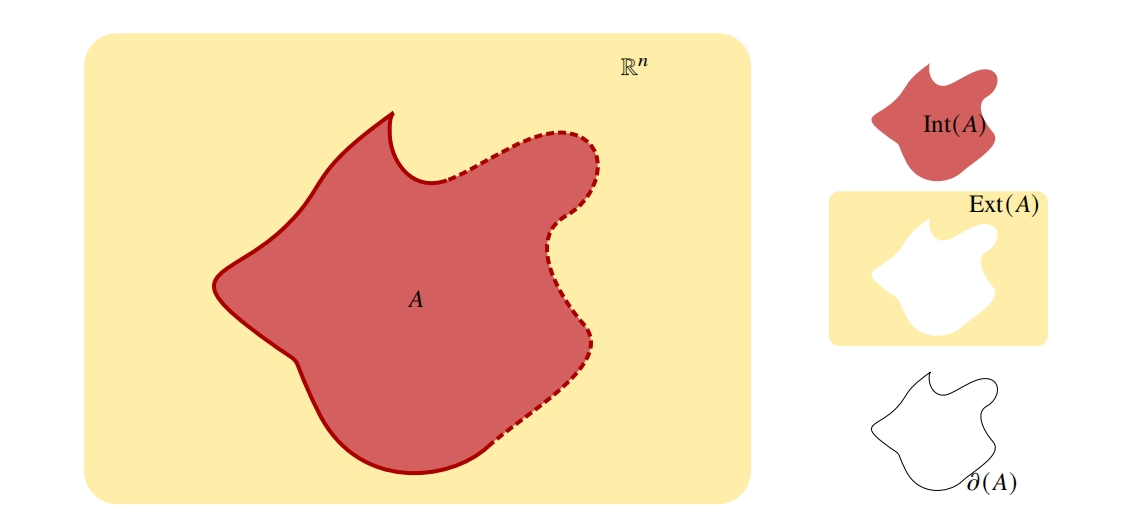
\includegraphics[width=0.6\textwidth]{figure/topological_space/int_ext_boundary.png}
    \caption{}
\end{figure}

By the following proposition, we can know closure and interior are closely related.

\begin{proposition}{}{}
   If $A=B^c$, then $\overline{A} = (\text{Int}(B))^c$.
\end{proposition}

\begin{proposition}{}{}
    (1) If $A\subset B$, then $\overline{A}\subset \overline{B}$;\\
    (2) $\overline{A}$ is the smallest closed subset of $X$ containing $A$;\\
    (3) $\overline{A}$ is the intersection of all closed sets of $X$ containing $A$;\\
    (4) $\overline{A}=A$ iff $A$ is closed;\\
    (5) $\overline{A\cup B}=\overline{A}\cup\overline{B}$;\\
    (6) $\overline{A\cap B}\subset \overline{A}\cap \overline{B}$.
\end{proposition}

\begin{example}{}{}
    Let $X=\{a,b,c,d,e\}$ and
    \begin{align*}
        \tau=\{X,\O,\{a\},\{c,d\},\{a,c,d\},\{b,c,d,e\}\}. 
    \end{align*} 
    Show that $\overline{\{b\}} = \{b,e\}$. 
\end{example}



\begin{definition}{}{}
    Let $A$ be a subset of a topological space $(X,\tau)$. Then $A$ is said to be dense in $X$ if $\overline{A}=X$.
    $X$ is said to be separable if there exists countable dense subset in $X$.
\end{definition}

\begin{proposition}{}{}
   Let $A$ be a subset of a topological space $(X,\tau)$. Then $A$ is dense in $X$ iff every non-empty open subset of $X$ intersects $A$ non-trivially, i.e.
   if $U\in \tau$ and $U\neq \O$ then $A\cap U\neq \O$. 
 \end{proposition}


\begin{example}{}{}
    $(X,\tau_d)$ is separable iff $X$ is countable. 
\end{example}
refer to \href{https://astarmathsandphysics.com/university-maths-notes/topology/2198-proof-that-a-discrete-space-is-separable-if-and-only-if-it-is-countable.html}{website proof}.


\begin{example}{}{}
    $(X,\tau_t)$ is separable. 
\end{example}
Let $A$ be a countably infinite subset of $X$. By example\ref{exa:limit point in trival topology}, 
$\overline{A}$ = $X$. Hence, $A$ is dense in $X$ and so $X$ is separable.
\begin{example}{}{}
    $(X,\tau_f)$ is separable.
\end{example}
    Let $A$ be a countably infinite subset of $X$. By example\ref{exa:limit point in cofinite topology}, 
    $\overline{A}$ = $X$. Hence, $A$ is dense in $X$ and so $X$ is separable.

\begin{example}{}{}
    $(X,\tau_c)$ is inseperable. 
\end{example}
    Let $A$ be a countably infinite subset of $X$.By example\ref{exa:limit point in cocountable topology},
    $\overline{A}$ = $A$. Hence, $X$ have no countably dense subset and so inseperable.

\begin{example}{}{}
    $(\R,\tau_e)$ is separable.
\end{example}
prove that $\overline{\Q}$=$\R$.


\subsection{Sequence convergence}
\begin{definition}{}{sequence convergence in topological space}
    Let $(X,\tau)$ be a topological space and $A$ a subset of $X$. Let $(x_n)_{n\in\N}$ be an infinite sequence in $A$.
    Then $(x_n)$ converages to the limit $x\in X$(denoted by $x_n\rightarrow x$) iff
    \begin{align*}
        \forall U\in \tau \text{ with }  x\in U \Rightarrow \{n\in \N:x_n\notin U\} \text{ is finite}.
    \end{align*}
    Or, 
    \begin{align*}
        \forall U\in \tau \text{ with }  x\in U \Rightarrow \exists N\in \N, \forall n>N, x_n\in U.
    \end{align*}
\end{definition}

In euclidean space,  the convergence point of a convergent sequence is unique and when $x$ is the limit point of the set $A$, there is a sequence $(x_n)$ in A, which converges to $x$. 
However, In general topological space, some difference appear.
\begin{proposition}{}{sequence convergence in cofinite topology}
    Let $(x_n)$ be a sequence which elements are different in $(R,\tau_f)$, then $\forall x\in X$, $x_n\rightarrow x$. 
\end{proposition}
\begin{proof}
    $\forall U\in \tau \text{ with }  x\in U \Rightarrow \{n\in \N:x_n\notin U\}= \{n\in \N:x_n\in U^c\} \text{ is finite}$.
\end{proof}
\begin{proposition}{}{sequence convergence in cocountable topology}
    Let $(x_n)$ be a sequence which elements are different in $(R,\tau_f)$, then
    \begin{align*}
        x_n\rightarrow x \Leftrightarrow \exists N\in\N, \forall n>N, x_n=x. 
    \end{align*}
\end{proposition}
\begin{proof}
    ($\Leftarrow$) clear by definition\ref{def:sequence convergence in topological space}
    \\
    ($\Rightarrow$) Consider the set $B:= \{x_n: x_n\neq x\}$. Since a sequence is countable, $B$ is countable. By example\ref{exa:limit point in cocountable topology}, B is closed.
    By construction, $x\notin B$, so $U=X\setminus B$ is an open set containing $x$. 
    But $x_n\rightarrow x$, so a tail of this sequence must lie in $X\setminus B$. Since $\{x_n\}\cap (X\setminus B)=\{x\}$, 
    this means that a tail of this sequence is constanst.  
\end{proof}

\section{Subspace}
\begin{definition}{}{}
    Let $A$ be a non-empty subset of a topological space $(X\,\tau)$. 
    The collection 
    \begin{align*}
        \tau_{A}=\{O\cap A: O\in \tau\}
    \end{align*}
    of subsets of $A$ is a topology on $A$ called the subspace topology
    (or the topology induced on $A$ by $\tau$). The topological space $(A,\tau_A)$ is said to be a subspace of $(X,\tau)$.
\end{definition}
Let's check that $\tau_A$ is indeed a topology on $A$.\\
(1) $A=X\cap A, \O = \O\cap A$, then $A,\O\in \tau_A$.\\
(2) If $U_{\alpha}\in \tau_A$, then $\cup_{\alpha}{U_\alpha} = \cup_{\alpha} (O_{\alpha}\cap A)=(\cup_{\alpha} O_{\alpha})\cap A\in\tau_A$.\\
(3) If $U_1,U_2\in\tau_A$, then $U_1\cap U_2 = (O_1\cap A)\cap (O_2\cap A)=(O_1\cap O_2)\cap A\in \tau_A$.

In the following content,  we follow the convention: a subset of topological Spaces is treated as a subspace. 
\par
Let $(X,\tau)$ be a topological space and $B\subseteq A\subseteq X$. Then
\begin{align*}
    (\tau_A)_B = & \{K\cap B:K\in \tau_A\} \\
        =  &\{(O\cap A)\cap B: O\in\tau\} \\
        =  &\{(O\cap B)\cap (A\cap B): O\in \tau\}\\
        \overset{B\subseteq A}{=}  &\{(O\cap B)\cap B: O\in \tau\}\\
        =  &\{(O\cap B): O\in \tau\}\\
        =  &\tau_B.
\end{align*}
Hence, there are two way to induce the topology on $B$: induced by the topology on $A$ or
induced by the topology on $X$.

\begin{example}{}{}
    Let $X=\{a,b,c,d,e,f\}$, 
    \begin{align*}
        \tau = \{X,\O, \{a\}, \{c,d\}, \{a,c,d\}, \{b,c,d,e,f\}\},
    \end{align*}
    and $A=\{b,c,e\}$. Then the subspace topology on $A$ is 
    \begin{align*}
        \tau_A = \{A,\O, \{c\}\}.
    \end{align*}
\end{example}


Consider the subset $[1,2]$ of $(\R,\tau_e)$. Then the topology on $[1,2]$ is 
\begin{align*}
    \tau = \{(a,b)\cap [1,2]: (a,b)\in \tau_e\}.
\end{align*}
\par
But here we see some surprising things happening; e.g.
$[1,\frac{3}{2})$ is certainly not an open set in $\R$, but $[1,\frac{3}{2})=(1,\frac{3}{2})\cap [1,2]$, is an open set in the subspace $[1,2]$.
\par
Also $(1,2]$ is not open in $\R$ but is open in $[1,2]$. Even $[1,2]$ is not open in $\R$, but is an open set in $[1,2]$.
\par
So whenever we speak of a set being open we must make perfectly clear in what space or what topology it is an open set. 

\begin{proposition}{}{closed intersection}
    Let $(X,\tau)$ be a topological space and $C\subset A\subset X$, then
    \begin{align*}
        C \text{ is closed in } A\Leftrightarrow C = A\cap V, \text{ where $V$ is closed in $X$}.  
    \end{align*}
\end{proposition}
\begin{proof}
    % \begin{align*}
    %     C \text{ is closed in } A &\Leftrightarrow A\setminus C \text{ is open in } A &\\
    %     & \Leftrightarrow \exists O\in \tau_{X}, \text{ s.t. } A\setminus C = O\cap A &\\
    %     & \Leftrightarrow \exists O\in \tau_{X}, C && = A\setminus(O\cap A) = (A\setminus O) \cup (A\setminus A) = &\\
    %     & &(A\setminus O) \cup \O = A\setminus O\\
         
    % \end{align*}

    \begin{align*}
        C \text{ is closed in } A &\Leftrightarrow A\setminus C \text{ is open in } A\\
         &\Leftrightarrow \exists O\in \tau_{X}, \text{ s.t. } A\setminus C = O\cap A\\
         &\Leftrightarrow \exists O\in \tau_{X}, C= A\setminus(O\cap A) \\
         &\quad\quad = (A\setminus O) \cup (A\setminus A)\\
         &\quad\quad = (A\setminus O) \cup \O = A\setminus O\\
         &\quad\quad = (A\cap X)\setminus O\\
         &\quad\quad = A\cap (X\setminus O)\\
         &\quad\quad = A\cap V, \text{ where $V$ is closed in $X$.}
        \end{align*}
\end{proof}

\begin{proposition}{}{}
    Let $(X,\tau)$ be a topological space, $B\subset A\subset X$, then\\
    (1) If $B$ is open(closed) in $X$, then $B$ is open(closed) in $A$;\\
    (2) If $A$ is open(closed) in $X$ and $B$ is open(closed) in $A$, then $B$ is open(closed) in $X$.
\end{proposition}
\begin{proof}
    (1) We know that $B=B\cap A$. If $B=O$ , then $B = O\cap A$ and so $B$ is open in $A$. 
    If $B$ is closed in $X$, by proposition\ref{prop:closed intersection}, $B=X\cap V$, where $V$ is closed in $X$. 
    Then $B=B\cap A = (X\cap V)\cap A = (X\cap A)\cap V$, by by proposition\ref{prop:closed intersection}, $B$ is closed in $A$.\\
    (2) If $B = O_1\cap A$ and $A=O_2$ , then $B=O_1\cap O_2\in \tau$ and so $B$ is open in $X$.
    If $A$ is closed in $X$ and $B$ is closed in $A$, then $A = X\cap V_1, B=A\cap V_2$, where $V_1,V_2$ is closed in $X$.
    Then, $B = X\cap (V_1\cap V_2)$. As $V_1\cap V_2$ is closed in $X$, $B$ is closed in $X$. 
\end{proof}

\section{Reference}
\begin{itemize}
    \item \href{https://www.ms.uky.edu/~guillou/F14/551Notes-Week4.pdf}{lecture notes from uky}
\end{itemize}
\section{Exercise}


\chapter{Continuous Mappings and Homeomorphisms}\label{1_2}

\section{Continuous Mappings}
We are already familiar with the notion of a continuous function from $\R$ to $\R$.
\par
A function $f:\R\rightarrow \R$ is said to be continuous at $x_0\in \R$ iff each positive real number $\epsilon$, 
there exists a positive real number $\delta$ such that $|f(x)-f(x_0)|<\epsilon$ when $|x-x_0|<\delta$. 
\par
It is not all obvious how to generalize this definition to general topological spaces where we do not have 
"absolute value" or "subtraction". So we shall seek another(equivalent) definition of continuity which lends itself more to 
generalization. 

It is easily seen that: $f:\R\rightarrow \R$ is continuous at $x_0\in\R$ iff for each interval $(f(x_0)-\epsilon, f(x_0)+\epsilon)$, 
for $\epsilon>0$, there exists a $\delta>0$ such that $f(x)\in(f(x_0)-\epsilon, f(x_0)+\epsilon)$ for all $x\in(x_0-\delta,x_0+\delta)$.
\par
This definition is an improvement since it does not involve the concept "absolute value" but it still involves "substraction". 
The next definition shows how to avoid substraction.

\begin{definition}{}{continuity definition}
    Let $(X,\tau)$ and $(Y,\tau')$ be topological spaces and $f$ a function from $X$ into $Y$.
    Then $f$ is continuous at $x_0\in X$ iff
    for each $U\in \tau'$ containing $f(x_0)$, there exists $K\in\tau$ containing $x_0$, such that $f(K)\subseteq U$.
\end{definition}
Use neighborhood to describe
\begin{proposition}{}{}
    Let $(X,\tau)$ and $(Y,\tau')$ be topological spaces and $f$ a function from $X$ into $Y$.
    Then $f$ is continuous at $x_0\in X$ iff for any neighborhood $N$ of $f(x_0)$ in $Y$, $f^{-1}$ is the neighborhood of $x_0$.
\end{proposition}
\begin{proof}
    
\end{proof}
\begin{definition}{}{}
    Let $(X,\tau)$ and $(Y,\tau')$ be topological spaces and $f$ a function from $X$ into $Y$.
    Then $f$ is continuous iff for each $x_0\in X$ and for each $U\in \tau'$ containing $f(x_0)$, 
    there exists $K\in\tau$ containing $x_0$, such that $f(K)\subseteq U$.
\end{definition}

As in analysis, continuity is a local concept. 
\begin{proposition}{}{}
    Let $(X,\tau)$ and $(Y,\tau')$ be topological spaces and $f$ a function from $X$ into $Y$ , $A$ a subset of $X$ and $x_0\in A$.
    We define the restriction of $f$ on $A$ as $f_A = f|A:A\rightarrow Y$, then\\
    (1) If $f$ is continuous at $x_0$, then $f_A$ is continuous at $x_0$.\\
    (2) When $A$ is open in $X$, if $f_A$ is continuous at $x_0$, then $f$ is continuous at $x_0$.
\end{proposition}

\begin{proof}
    (1) We need to prove for each $U\in \tau'$ with $f_A(x_0)\in U$, there exists $O\in \tau_A$ with $x_0\in O$, $f_A(O)\subseteq U$.
    $f$ is continuous at $x_0$ and $x_0\in A$, then for each $U\in \tau'$ with $f(x_0)=f_A(x_0)\in U$, there exists $K\in \tau$ with $x_0\in K$, $f(K)\subseteq U$.
    Since $A\cap K\in \tau_A$ with $x_0\in A\cap K$ and $f_A(A\cap K) = f(A\cap K)\subseteq f(A)\cap f(K)\subseteq Y\cap U= U$. Hence, $f_A$ is continuous at $x_0$.
    \par
    (2) $f_A$ is continuous at $x_0$, then for each $U\in\tau'$ containing $f_A(x_0)=f(x_0)$, there exists $(K\cap A)\in \tau_A$($K\in\tau$) containing $x_0$, 
    such that $f_A(K\cap A)\subseteq U$. Since $A\in \tau$, $K\cap A\in \tau$ and $f(A\cap K)=f_A(A\cap K)\subset U$. Hence, $f$ is continuous at $x_0$. 
\end{proof}


\begin{definition}{}{}
    Let $f$ be a function from a set $x$ into a set $Y$. If $S$ is any subset of $Y$, 
    then the set $f^{-1}(S)$ is defined by
    \begin{align*}
        f^{-1}(S) = \{x:x\in X \text{ and } f(x)\in S\}.
    \end{align*}
    Then subset $f^{-1}(S)$ of $X$ is said to be the inverse image of $S$.
\end{definition}
\begin{remark}
    Note that an inverse function of $f$ exists iff $f$ is bijective. 
    But the inverse image of any subset of $Y$ exists even if $f$ is neither one-to-one nor onto.
\end{remark}

\begin{proposition}{}{}
    Let $f$ be a mapping of a topological space $(X,\tau)$ into a topological space $(Y,\tau')$. Then the following conditions are equivalent:\\
    (1) $f$ is continuous;\\
    (2) for each $U\in\tau'$, $f^{-1}(U)\in \tau$;\\
    (3) for each closed set $V$ in $Y$, $f^{-1}(Y)$ is closed in $X$.
\end{proposition}

\begin{proof}
    
\end{proof}

In $(\R,\tau_e)$, we can use sequence convergence to characterize continuity, 
but in general topological space, we cannot do this.
\begin{proposition}{}{continuity means sequentially continous}
    $f:X\rightarrow Y$ is continuous at $x_0\in X$, then $x_n\rightarrow x_0$ implies $f(x_n)\rightarrow f(x_0)$.
\end{proposition}
\begin{proof}
    $f$ is continous at $x_0\in X$ and $x_n\rightarrow x_0$, 
    then $\forall U\in\tau_Y$ containing $f(x_0)$, 
    there exists $K\in\tau_X$ containing $x_0$ such that $f(K)\subseteq U$.
    Since $x_n\rightarrow x_0$, $\exists N\in\N$, $\forall n>N$, $x_n\in K$, then $f(x_n)\in f(K)\subseteq U$.
    So $f(x_n)\rightarrow f(x_0)$.
\end{proof}
However, the inverse proposition is not true. 
Let $f:X\rightarrow Y$ be injective, $X$ be a uncountable space with $\tau_c$ and $Y$ be a discrete space.
Then, by proposition\ref{prop:sequence convergence in cocountable topology}, 
When $x_n\rightarrow x_0$ in $X$, $\exists N\in N$, $\forall n>N$, $x_n=x$, 
then $f(x_n)=f(x)$ and so $f(x_n)\rightarrow f(x)$.
But $f$ is not continuous at $x_0$, because for $U=\{f(x_0)\}\in \tau_Y$ containing $f(x_0)$, 
$\forall K\in \tau_X$ containing $x_0$, $f(K)\supset \{f(x_0)\}$ as $f$ is injective and $K\supset \{x_0\}$.


\section{The properties of continuous mapping}

Firstly, we introduce some simple and common continuous mappings.
\begin{proposition}{}{}
    Identity mapping $\text{id}:X\rightarrow X$ is continuous.
\end{proposition}

\begin{definition}{}{Inclusion mapping}
        Let $X$ be a topological space and $A\subset X$. 
        Then inclusion mapping $i_A:A\rightarrow X$ is the mapping defined as:
        \begin{align*}
            i_A:A\rightarrow X: \forall x\in A:i_{A}(x)=x
        \end{align*}
\end{definition}

\begin{proposition}{}{}
    Let $X$ be a topological space and $A\subset X$. 
    Then inclusion mapping $i_A:A\rightarrow X$ is continuous.
\end{proposition}

\begin{proof}
    For any open set $U$ in $X$, $i^{-1}(U)=U\cap A$ is open in $A$.
\end{proof}

\section{Homemorphism}

\begin{definition}{}{}
    Let $(X,\tau)$ and $(Y,\tau')$ be topological spaces, 
    and let $f:X\rightarrow Y$ be a bijection. 
    $f$ is said to be a homeomorphism if $f$ is continous and its inverse $f^{-1}$ is continous.\\
    In this case we say that $(X,\tau)$ and $(Y,\tau')$ are homeomorphism, and write $(X,\tau)\cong (Y,\tau')$, or
    more often simply $X\cong Y$ if the topologies are understood from context.
\end{definition}

\begin{proposition}{}{}
    Let $(X,\tau)$ and $(Y,\tau')$ be a topological spaces, and let $f:X\rightarrow Y$ be a bijection, 
    Then the following are equivalent.\\
    (1) $f$ is a homeomorphism.\\
    (2) $f$ is continous and open.\\
    (3) $f$ is continuous and closed.\\
    (4) $U\subset X$ is open iff $f(U)\subset Y$ is open.
\end{proposition}

\begin{definition}
    Let $X$ and $Y$ be topological spaces. 
    Suppose $f:X\rightarrow Y$ is an injective continous mapping. 
    If the function $f':X\rightarrow f(X)$ obtained by restricting the range of $f$ is a homeomorphism, 
    then the map $f:X\rightarrow Y$ is called a topological embedding.
\end{definition}

\section{Exercise}

\begin{exercise}{}{}
    Let $f$ be a mapping from $X$ to $Y$, the following statements are equivalent:\\
    (1) $f$ is continous;\\
    (2) $\forall A\subseteq X$, $f(\overline{A})\subset \overline{f(A)}$;\\
    (3) $\forall B\subseteq Y$, $\overline{f^{-1}(B)}\subset f^{-1}(\overline{B})$.
\end{exercise}

\begin{proof}
    (1)$\Rightarrow$(2): $f$ is continous. Since $\overline{f(A)}$ is closed in $Y$, 
    then $f^{-1}(\overline{f(A)})$ is closed in $X$. Since $f(A)\subseteq \overline{f(A)}$, 
    $A\subseteq f^{-1}(\overline{f(A)})$. Since $\overline{A}$ is the smallest closed set containing $A$, 
    $\overline{A}\subseteq f^{-1}(\overline{f(A)})$. Then, $f(\overline{A})\subseteq f(f^{-1}(\overline{f(A)}))\subseteq \overline{f(A)}$.

\end{proof}

\begin{exercise}{}{}
    $f:X\rightarrow Y$ is called open(closed) mapping, if $f(X)$ is open(closed). 
    Illustrate that open mapping may not be closed mapping and vice versa.
\end{exercise}
\begin{proof}
    
\end{proof}

\begin{exercise}
    If $f:X\rightarrow Y$ is bijective, then
    \begin{align*}
        f \text{ is open mapping }\Leftrightarrow f\text{ is closed mapping }\Leftrightarrow f^{-1} \text{ is continuous}.
    \end{align*}
\end{exercise}

\begin{proof}
    $\forall U\in\tau_X$,
    \begin{align*}
        f(U)\in \tau_Y \Leftrightarrow & Y\setminus f(U) \text{ is closed }\\
                                \overset{f \text{ is bijective }}{\Leftrightarrow} & f(X\setminus U) \text{ is closed } \\
                                \Leftrightarrow & f \text{ is closed mapping}.
    \end{align*}
    Since $f$ is bijective, $f^{-1}$ exists. As $f$ is open mapping, $f^{-1}$ is continuous.
\end{proof}

\begin{remark}
    From this exercise, we can know if $f$ is bijective, continuous and open, then $f$ is homeomorphism.
\end{remark}

\section{Reference}

\begin{itemize}
    \item \href{https://raphaeltinarrage.github.io/files/EMAp/Lesson2.pdf}{Homeomorphisms}
    \item 
\end{itemize}



\newcommand{\ob}{\overline{\mathcal{B}}}
\chapter{Topological basis and Product Space}\label{chp:1_3}


\section{Topological basis}
Let's recall the euclidean topology in $\R$, 
\begin{align*}
    \tau_e = \{U : U=\cup_{(a,b)\in I} (a,b), a<b\in \R, I \text{ is a collection of open interval}\}.
\end{align*}
It seems like the entire collection of sets
in $\tau_e$ can be specified by declaring that just the usual open intervals are open. Once these
“special sets” are known to be open, we get all the other sets for free by taking unions.
These special collections of sets are called bases of topologies.

\begin{definition}{}{basis for given topology definition}
    Let $(X,\tau)$ be a topological space. 
    A collection $\mathcal{B}$ of subsets of $X$ is said to be a basis for the topology $\tau$
    if for each $U\in \tau$, $U=\cup_{B\in I} B$, where $I\subseteq \mathcal{B}$.
\end{definition}

If we construct a set $\ob=\{U_{B\in I}B: I \subseteq \mathcal{B}\}$, 
then we can get a improved definition. 

\begin{definition}{}{basis for given topology definition}
    Let $(X,\tau)$ be a topological space. 
    A collection $\mathcal{B}$ of subsets of $X$ is said to be a basis for the topology $\tau$
    if $\ob=\tau$.
\end{definition}

\begin{proposition}{}{}
    Let $(X, \tau)$ be a topological space.
     A collection $\mathcal{B} \subseteq \mathcal{P}(X)$ is a
basis for $\tau$ if and only if\\
(1) $\mathcal{B} \subseteq \tau$,\\
(2) for any $U \in \tau$ and any $x \in U$, there exists $B \in \mathcal{B}$ such that $x \in B \subseteq U$.
\end{proposition}

\begin{proof}
    ($\Rightarrow$): Suppose $\ob=\tau$, then $\mathcal{B}\subseteq \ob\subseteq \tau$. 
    Since $\tau\subseteq \ob$, then take $B=U$, $x\in B\subseteq U$.
    \\
    ($\Leftarrow$): (1) implies $\ob\subseteq \tau$, 
    (2) implies $U\subseteq \cup_{B_x}B_x\subseteq U$ and so $U=\cup_{B_x}B_x\in \ob$. 
    Hence, $\ob\subseteq \tau$ and so $\ob=\tau$.
\end{proof}

\begin{example}{}{}
    $\mathcal{B}=\{(a,b):a,b\in\R,a<b\}$ is a basis for $(\R,\tau_e)$.
\end{example}

\begin{example}{}{}
    $\mathcal{B}=\{\{x\}:x\in X\}$ is a basis for $(X,\tau_s)$. 
\end{example}

Observe that $\tau=\mathcal{P}(X)$ is also a basis for the discrete topology on $X$. 
Therefore, there can be many different bases for the same topology. indeed if $\mathcal{B}$ is a basis for a topology $\tau$ on a set $X$ and $\mathcal{B}_1$ is a collections of subsets of $X$ such that $\mathcal{B}\subseteq \mathcal{B}_1\subseteq \tau$, then $\mathcal{B}_1$ is also a basis for $\tau$.


The above content show us when $\mathcal{B}$ is basis for a given topology in $X$. 
Now we consider when $\mathcal{B}$ is basis for a topology in $X$.

\begin{proposition}{}{}
    Let $X$ be a non-empty set and $\ob$ be a collection of subsets of $X$. Then $\mathcal{B}$ is a basis for a topology on $X$ iff
    $\overline{B}$ is a topology.
\end{proposition}


\begin{proposition}{Basis for a topology}{}
    Let $X$ be a non-empty set and $\mathcal{B}$ be a collection of subsets of $X$. Then $\mathcal{B}$ is a basis for a topology on $X$ iff $\mathcal{B}$ has the following properties:\\
    (1) $X=\cup_{B\in \mathcal{B}}B$, and\\
    (2) for any $B_1,B_2\in \mathcal{B}$, $B_1\cap B_2=\cup_{B\in I}B$, where $I\subseteq\mathcal{B}$.
\end{proposition}

\begin{proof}
($\Rightarrow$): $\ob$ is a topology, then $X\in \ob$ and so $X=\cup_{B\in I}B$.
Since $B\in\mathcal{B}$ is contained in $X$, $X\subseteq \cup_{B\in\mathcal{B}}\subseteq X$. Hence, $X=\cup_{B\in\mathcal{B}}B$.
If $B_1,B_2\in\mathcal{B}$, then $B_1,B_2\in\ob$ and so $B_1,B_2$ is open. Then $B_1\cap B_2$ is open and so contained in $\ob$. 

($\Leftarrow$): We should show that $\ob$ is a topology. By (1), $X\in\ob$. 
$\O$ is the empty union of members in $\ob$. Hence, $\O\in\ob$. For $U_J=\{U\in J: J\subseteq\ob\}$, $U$ is the union of members in $\mathcal{B}$.
Then $\cup_{U\in U_J} U$ is the union of members in $\mathcal{B}$ and so belong to $\ob$. 
If $U_1,U_2\in \ob$, then $U_1=\cup_{B_1\in I_1}B_1, U_2=\cup_{B_2\in I_2}B_2$.
Then $U_1\cap U_2 = (\cup_{B_1\in I_1}B_1)\cap (\cup_{B_2\in I_2}B_2)=\cup_{B_1\in I_1}(B_1\cap (\cup_{B_2\in I_2}B_2))= \cup_{B_1\in I_1,B_2\in I_2}(B_1\cap B_2)$. 
By (2), $B_1\cap B_2$ is the union of members in $\mathcal{B}$, thus $U_1\cap U_2$ is the union of members in $\mathcal{B}$ and so contained in $\mathcal{B}$.
Hence, $\ob$ is a topology.
\end{proof}

\textcolor{red}{Haven't done! Add the content about basis for a given topology.}

\section{Product space}


\part{Topology Invariant}
\chapter{THE AXIOMS OF COUNTABILITY
}\label{chp:2_1_1}

Now we turn to countability features in topology. In topology, an axiom of countability is a topological property that asserts the existence of a countable set with certain
properties. There are several different topological properties describing countability.

\section{First countable spaces}

\begin{definition}{}{}
    Let $(X,\tau)$ be a topological space and $x$ be an element of $X$.
    A neighborhood base at $x$ is a set $\mathcal{U}$ of neighborhood $N$ of $x$ such that:
    \begin{align*}
        N\text{ is a neighborhood of }x\Rightarrow \exists U\in\mathcal{U}:U\subseteq N.
    \end{align*}
\end{definition}

\begin{definition}{}{}
    A topological space $(X,\tau)$ is called first countable, or an $C_1$ space, if 
    for every point in $X$ has a countable neighborhood base, i.e.
    for each $x\in X$, there exists a countable family $\mathcal{U}=\{U_i^x:i\in\N\}$, where $U_i^x$ is neighborhood of $x$,
    such that every neighborhood $N$ of $x$, there exists $n$ \text{s.t.} $U_n^x\subseteq N$.
\end{definition}


Here are some examples of $C_1$-spaces and non-$C_1$-spaces.

\begin{example}{}{}
    Any metric space is first countable since we can take $U_n^x=B(x,\frac{1}{n})$.
\end{example}

\begin{example}{}{}
    $(\R,\tau_c)$ is not first countable: for any countable family $\mathcal{U}=\{U_i^x:i\in\N\}$ of open sets containing $x$,
    $\cup_{U\in\mathcal{U}}U^c$ is countable. Take $y\notin \cup_{U\in\mathcal{U}}U^c$ and $y\neq x$, then $\forall U\in\mathcal{U}, y\in U$. 
    Then $\R\setminus\{y\}$ is a open set containing x, but it doen't contain any $U\in\mathcal{U}$. 
\end{example}


\begin{example}{}{}
    $(\R,\tau_f)$ is not first countable.
\end{example}

\begin{proposition}{}{Decrement countable neighborhood base}
    Let $(X,\tau)$ be a topological space. If $x\in X$ has a countable neighborhood base $\mathcal{U}=\{U_i^x\}$,
    then $x$ has a countable neighborhood base $\{V_i^x\}$ , which satisfys $V_m^x\subset V_n^x$ when $m>n$.
\end{proposition}
\begin{proof}
    If one has a countable neighborhood base $\{U_i^x:i\in\N\}$ at $x$, then one can take
    Then $\{V_i^x:i\in\N\}$ is countable. 
    $V_n^x=\cap_{n}U_n^x$. Since $V_n^x\subset U_n^x$, $\{V_i^x:i\in\N\}$ is a neighborhood base at $x$ and $V_m^x\subset V_n^x$ when $m>n$.
\end{proof}

\begin{proposition}{}{fc closure sequential convergence}
    Let $(X,\tau)$ be first countable and $A$ a subset of $X$, then
    \begin{align*}
        x\in\overline{A}\Leftrightarrow \exists \{x_n\}\subset A, \text{ s.t. } x_n\rightarrow x.
    \end{align*}
\end{proposition}

\begin{proof}
    ($\Rightarrow$): By propsition\ref{prop:Decrement countable neighborhood base}, we can take a countable neighborhood base $\{V_i^x\}$ which 
    satisfys $V_m\subseteq V_n$ when $m>n$. Since $x\in A$, by the property of closure, $V_n\cap A\neq \O$.
    We take $x_n\in V_n\cap A$, then we get a sequence $\{x_n\}\subset A$. 
    Since $\{V_n^x\}$ is a neighborhood base, for any neighborhood $U^x$ of $x$, there exsits $n$ such that $x\in V_n^x\subseteq U^x$. 
    Then $\forall m\geqs n$, $V_m^x\subseteq U^x$. 
    Then $\forall m\geqs n$, $x_m\in U^x$. By definition\ref{def:sequence convergence in topological space}, $x_n\rightarrow x$.
\end{proof}

\begin{corollary}{}{}
    Let $(X,\tau)$ be first countable and $A$ a subset of $X$, then
    \begin{align*}
        A \text{ is closed }&\Leftrightarrow \text{for any sequence }\{x_n\}\subset A \text{ with } x_n\rightarrow x, \text{one has } x\in A.\\
        & i.e. A \text{ contains all its sequential limits.}
    \end{align*}
\end{corollary}

\begin{proof}
    ($\Rightarrow$): If $A$ is closed, then $A$ contains all its limits including sequential limits.\\
    ($\Leftarrow$): $\forall x\in \overline{A}$, by proposition\ref{prop:fc closure sequential convergence},
    $\exists \{x_n\}\subset A$, s.t. $x_n\rightarrow x$. Then by the condition, $x\in A$. Then, $\overline{A}\subseteq A$.
    Since $A\subseteq \overline{A}$, $A=\overline{A}$ and so $A$ is closed. 
\end{proof}

\begin{corollary}{}{}
    Suppose $(X,\tau)$ is first countable and $f$ is a map from $X$ to $Y$.
    \begin{align*}
        f:X\rightarrow Y \text{ is continuous at } x_0\in X \text{ iff } x_n\rightarrow x_0 \text{ implies } f(x_n)\rightarrow f(x_0).
    \end{align*}
\end{corollary}
\begin{proof}
    ($\Rightarrow$): proof of proposition\ref{prop:continuity means sequentially continous}.\\
    ($\Leftarrow$): Suppose $f$ is not continous at $x_0$. Then there exists a open set $U$ containing $f(x_0)$, 
    for all open set $K$ containing $x_0$, $f(K)\not\subseteq U$, which means $K\cap (f^{-1}(U))^c\neq \O$. 
    Then by the property of closure, $x_0\in \overline{(f^{-1}(U))^c}$. Then by proposition \ref{prop:fc closure sequential convergence}, 
    $\exists \{x_n\}\in \overline{(f^{-1}(U))^c}$, $x_n\rightarrow x$. Then by the condition, $f(x_n)\rightarrow f(x_0)$.
    Then by the definition of convergent sequence, all most $f(x_n)\in U$. But $f(x_n)\in f(\overline{(f^{-1}(U))^c})\subseteq \overline{f((f^{-1}(U))^c)}= \overline{f(f^{-1}(U^c))}\subseteq \overline{U^c}$, a contradiction.
    Hence, $f$ is continuous at $x_0$.
\end{proof}

\section{Second countable spaces}

\begin{definition}{}{}
    A topological space $(X,\tau)$ is called second countable, or an $C_2$ space, if 
    it has a countable topological base, i.e.
    there exists a countable family $\{U_i\}$ of open sets such that, for each $x\in X$, 
    every open set $U$ containing $x$, there exists $n$ \text{s.t.} $x\in U_n\subseteq U$.
\end{definition}

\begin{remark}
    In $C_1$, the open set family is related to $x$. 
    But, In $C_2$, the open set family doesn't need.
    Obviously any second countable space is a first countable space. But the converse
is not true, for example, $(\R, \tau_s)$ is first countable as it is a metric space, but it is
not second countable. Since every base for a discrete topology must include all singleton sets 
(since for each $x\in X$, the set $\{x\}$ is an open neighborhood of $x$, and so if $\mathcal{B}$
is any base for $X$, then there is a $B\in \mathcal{B}$ with $x\in B\subseteq \{x\}$, 
which implies $B={x}\in\mathcal{B}$). Since $\R$ is not countable, there is no a conntable family of open sets.
\end{remark}

\section{Separable spaces}

\begin{proposition}{}{second countable is separable}
    Any second countable topological space is separable.
\end{proposition}
\begin{proof}
    It is equivalent to prove the space has a coutable dense subset.
    Let $\{U_n:n\in\N\}$ be a countable basis of $(X,\tau)$. For each $n$, we choose a point $x_n\in U_n$ and let $A=\{x_n:n\in\N\}$. 
    Then $A$ is a countable subset in $X$. We claim that $\overline{A}=X$. In fact, 
    for any $x\in X$ and any open neighborhood $U$ of $x$, there exists $n$ s.t. $x\in U_n\subseteq U$. 
    In particular, $U\cap A\neq \O$. So we get $\overline{A}=X$.
\end{proof}

\begin{proposition}{}{}
    A metric sapce is second countable iff it is separable.
\end{proposition}

\begin{proof}
    ($\Rightarrow$): proof of proposition\ref{prop:second countable is separable}.\\
    ($\Leftarrow$): Suppose that $(X,d)$ is a separable metric space. Then $X$ has a countable dense subset $A$.
    So
    \begin{align*}
        \mathcal{B} = \{B(a,\frac{1}{n}):a\in A, n\in \N\}
    \end{align*} 
    is a countable family of open balls in $X$.
    Show that $\mathcal{B}$ is a base for the metric topology on $X$.
    In other words, show that if $U$ is a non-empty open set in $X$, and $x\in U$, then $\exists B\in \mathcal{B}$
    such that $x\in B\subseteq U$. 
    Since there is some $\epsilon>0$ such that $B(x,\epsilon)\subseteq U$;
    thus, you need only show that there is some $B(a,\frac{1}{n})\in \mathcal{B}$
    such that $x\in B(a,\frac{1}{n})\subseteq B(x,\epsilon)$.
    We take $n>\frac{2}{\epsilon}$ and $a\in A$ such that $d(x,a)<\frac{1}{n}$, which means $x\in B(a,\frac{1}{n})$.
    For $y\in B(a,\frac{1}{n})$, $d(a,y)<\frac{1}{n}$. Then $d(x,y)<d(x,a)+d(a,y)<\frac{2}{n}<\epsilon$. So $y\in B(x,\epsilon)$ and $B(a,\frac{1}{n})\subseteq B(x,\epsilon)$.
    Hence, $(X,d)$ has a countable topological base and so second countable.
\end{proof}



\section{Multiplicability and heritability}



\section{Reference}
\begin{itemize}
    \item \href{http://staff.ustc.edu.cn/~wangzuoq/Courses/21S-Topology/Notes/Lec13.pdf}{THE AXIOMS OF COUNTABILITY}
\end{itemize}



\chapter{SEPARATION AXIOMS}\label{chp:2_1_2}

\section{Four separation axioms}

By "separation axioms" we mean properties of topological spaces concerning separating certain disjoint sets via (disjoint) open sets. [Caution: It is very different from
the conception separable that we learned last time!] There are many different separations axioms 1
, four of them are used more often than the others, and we have seen
two of them which are most important:


\begin{definition}{}{}
    ($T_1$)
    \begin{align*}
        \forall x_1\neq x_2\in X,\exists \text{ open sets }U,K \text{ s.t. }\\
        x_1\in U\text{ but } x_2\notin U \text{ and } x_2\in K\text{ but } x_1\notin K. 
    \end{align*}
    ($T_2$)
    \begin{align*}
        \forall x_1\neq x_2\in X,\exists \text{ open sets } U,K \text{ s.t. }\\
        x_1\in U,x_2\in K \text{ and }U\cap K=\O.
    \end{align*}
    ($T_3$)
    \begin{align*}
        \forall \text{ closed sets }V \text{ and }x\notin V, \exists \text{ open sets } U,K \text{ s.t. }\\
        V\subset U, x\in K \text{ and } U\cap K=\O.
    \end{align*}
    ($T_4$)
    \begin{align*}
        \forall \text{ closed sets } V_1 \text{ and } V_2 \text{ with } V_1\cap V_2=\O, \exists \text{ open sets }\\
        U,K \text{ s.t. } V_1\subset U, V_2\subset K \text{ and }U\cap K=\O.
    \end{align*}
\end{definition}

\begin{figure}[htbp]
    \centering
    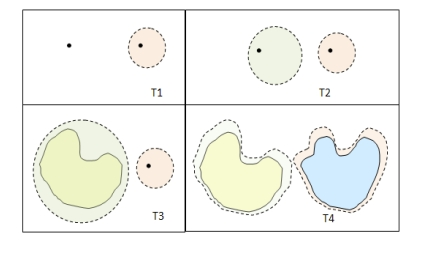
\includegraphics[width=0.6\textwidth]{figure/separation/separation_fig.png}
    \caption{}
\end{figure}

\begin{remark}
    In some books, "both (T1) and (T3)" in our sense means "regular" 
    "both (T1) and (T4)" means "normal"; in some other books, "(T3)" means "regular"
    and "(T4)" means "normal". In order to reduce ambiguity, we only talk about (T1-T4) in our sense
    but not "regular" and "normal". 

\end{remark}

\section{Equivalent characterizations}
First we give equivalent characterizations of these axioms.
\begin{proposition}{}{}
    Let $(X,\tau)$ be a topological space.\\
    (1) $(X,\tau)$ is (T1) iff any single point set is closed.\\
    (2) $(X,\tau)$ is (T2) iff the diagonal $\triangle =\{(x,x):x\in X\}$ is closed in $X\times X$.\\
    (3) $(X,\tau)$ is (T3) iff $\forall$ open set $U$ with $x\in U$, $\exists \text{ open set } K$ such that $x\in K\subset \overline{K}\subset U$\\
    (4) $(X,\tau)$ is (T4) iff $\forall$ closed set $V\subset U$($U$ is open), $\exists \text{ open set }K$ such that $V\subset K\subset \overline{K}\subset U$.
\end{proposition}

\begin{proof}
    (1) and (2) follow from definitions, while (3) and (4)
follow from open-closed duality:\\
(1) ($\Rightarrow$): For $\forall y\neq x$, $\exists U_y\in \tau$ such that $y\in U_y$ but $x\notin U$, then $U_y\subset \{x\}^c$ 
    and $\{x\}^c=\cup_{y\neq x}U_y$.
    is open, i.e. $\{x\}$ is closed. \\
    ($\Leftarrow$): For $\forall x\neq y$, take $U={y}^c$ and $K={x}^c$. Then $U,K$ is open and $x\in U, y\in K$ but $x\notin K, y\notin U$.\\
(2) The proof is trivial if $|X|=1$, assume that $|X|>1$.\\
    ($\Rightarrow$): 
    Suppose $X$ is Hausdorff. Let $(a,b)\in X\times X-\triangle$. 
    (Note that such an element exists, since $|X|>1$). Then, $a\neq b$.
    Since $X$ is Hausdorff, we can pick open sets $U_a$ and $U_b$ such that $a\in U_a,b\in U_b$ and $U_a\cap U_b=\O$.
    Now, note that $(U_a\times U_b)\cap \triangle = \O$ (If not, $\exists (p,q)\in (U_a\times U_b)\cap \triangle$. 
    Then $(p,q)\in \triangle$ and so $p=q$. But then $p\in U_a$ and $p\in U_b$, contradicting the fact that $U_a\cap U_b=\O$.)
    Since $U_a\times U_b\in \tau_{X\times X}$ and $(a,b)\in U_a\times U_b\subseteq X\times X-\triangle$, 
    by proposition\ref{prop:open set judging}, $X\times X-\triangle$ is open in $X\times X$. 
    Hence, $\triangle$ is closed in $X\times X$.\\
    ($\Leftarrow$): For $x\neq y\in X$, i.e. $(x,y)\in \triangle^c$, there exists $U,K$ such that $x\in U,y\in K$ and
    $(x,y)\in U\times K\subseteq \triangle^c$. 
    It follows $U\cap K=\O$, if not, there exists $z\in U\cap K$, 
    then $(z,z)\in U\times K\cap\triangle=\O$. This is a contradiction. 
    Hence, $X$ is Hausdorff.\\
(3) ($\Rightarrow$):
    $\forall$ open set $U$ with $x\in U$, then $x\notin U^c$ (closed set).
    Then, there exists $K_1,K_2\in \tau$ such that $x\in K_1, U^c\subset K_2$ and $K_1\cap K_2=\O$.
    Then by proposition\ref{prop:closure and interior relation}, $x\in K_1\subset \overline{K_1}\subset K_2^c\subset U$.\\
    ($\Leftarrow$):
    Suppose $x\notin V$ closed, i.e. $x\in V^c$ open, then there exists $K\in \tau$ such that 
    $x\in K\subset \overline{K}\subset V^c$. It follows $K\cap \overline{K}^c=\O$, $x\in K$ and $V\subset \overline{K}^c$.\\
(4) ($\Rightarrow$):
    Suppose closed $V\subset U$ open, then $V\cap U^c=\O$.
    So there exists $K_1,K_2\in\tau$ such that $K_1\cap K_2=\O, V\subset K_1$ and $U^c\subset K_2$.
    So $V\subset K_1\subset \overline{K_1}\subset K_2^c\subset U$.\\
    ($\Leftarrow$):
    Suppose $V_1,V_2$ are closed and $V_1\cap V_2=\O$. Then $V_1\subset V_2^c$ open. 
    So there exists $K\in \tau$ such that $V\subset K\subset \overline{K}\subset V_2^c$.
    It follows that $K\cap \overline{K}^c=\O$, $V\subset K$ and $V_2\subset \overline{K}^c$. 
\end{proof}


\section{Relations between different separation axioms}


We can also study the relations between these axioms. Obviously we have
\begin{proposition}{}{}
    (1) $T_2\Rightarrow T_1$.\\
    (2) $T_1+T_3\Rightarrow T_2, T_1+T_4\Rightarrow T_2, T_1+T_4\Rightarrow T_3$.\\
\end{proposition}

\begin{proof}
    (1) \begin{align*}
    \forall x_1\neq x_2\in X &\overset{T2}{\Rightarrow} \exists U,K\in \tau: x_1\in U,x_2\in K \text{ and } U\cap K=\O\\
                            & \Rightarrow x_1\in U, x\notin K \text{ and } x_2\in K, x_2\notin U\\
                            & \Rightarrow x_1\in U\setminus K \text{ and } x_2\in K\setminus U.
        \end{align*}
    (2) 
    \begin{align*}
        \forall x_1\neq x_2\in X &\overset{T1}{\Rightarrow} \{x_1\} \text{ is closed and } x_2\notin \{x_1\}\\
                                & \overset{T3}{\Rightarrow} \exists U,K\in \tau \text{ s.t. } \{x_1\}\subseteq U, x_2\in K \text{ and } U\cap K=\O.\\
                                & \Rightarrow x_1\in U,x_2\in K \text{ and } U\cap K=\O.
    \end{align*}
    \begin{align*}
        1
    \end{align*}
\end{proof}

\begin{proposition}{}{}
    A metric sapce satisfys $T_1,T_2,T_3 \text{ and } T_4$.
\end{proposition}

\section{Productive and hereditary}

\begin{proposition}{}{}
    $T_1$ is hereditary. 
\end{proposition}

\begin{proof}
    Let $(X,\tau)$ be a $T_1$ space and $A\subset X$. That is: 
    \begin{align*}
        \forall x\neq y\in A\subset X, \exists U,K\in\tau:\\
        x\in U\text{ but } y\notin U\text{ and } y\in K\text{ but } x\notin K.
    \end{align*}
    Then one can find
    \begin{align*}
        U_A := U\cap A, K_A:=K\cap A.
    \end{align*}
    It follows that $U_A,K_A\in \tau_A$ s.t. $x\in U_A$ but $y\notin U_A$ and $y\in K_A$ but $x\notin K_A$
\end{proof}


\begin{proposition}{}{}
    $T_2$ is hereditary. 
\end{proposition}

\begin{proof}
    Let $(X,\tau)$ be a $T_2$ space and $A\subset X$. That is: 
    \begin{align*}
        \forall x\neq y\in A\subset X, \exists U,K\in\tau:\\
        x\in U,y\in K\text{ and } U\cap K=\O.
    \end{align*}
    Then one can find
    \begin{align*}
        U_A := U\cap A, K_A:=K\cap A.
    \end{align*}
    It follows that $U_A,K_A\in \tau_A$ s.t. $x\in U_A$, $y\in K_A$ and $U_A\cap K_A=(U\cap A)\cap (K\cap A)=(U\cap K)\cap A=\O$.
\end{proof}

\begin{proposition}{}{T3 hereditary}
    $T_3$ is hereditary. 
\end{proposition}

\begin{proof}
    Let $(X,\tau)$ be a $T_3$ space and $A\subset X$. Then
    $\forall \text{ closed set } V$ in $A$ and $x\in A\setminus V$, by proposition\ref{prop:closed in subspace}, $\exists C$ which is closed in $X$ such that $V=A\cap C$.
    Also $x\notin C$. That is 
    $\exists U,K\in\tau$ s.t. $x\in U, C\subset K$ and $U\cap K=\O$. 
    Then one can find $U_A:= U\cap A, K_A:= K\cap A\in \tau_A$ s.t. $x\in U_A,V\subset K_A$ and $U_A\cap K_A=\O$.
\end{proof}

\begin{proposition}{}{}
    $T_4$ preserved in closed subspace.
\end{proposition}

\begin{proof}
    Let $(X,\tau)$ be a $T_4$ space and $A\subset X$ is closed.
    $\forall \text{ closed set } V_1,V_2$ in $A$ with $V_1\cap V_2=\O$, by corollary\ref{cor:closed transitive2}, 
    we can know that $V_1,V_2$ is closed in $X$ and $V_1\cap V_2=\O$. 
    Then $\exists U,K\in \tau$ s.t. $V_1\subset U, V_2\subset K$ and $U\cap K=\O$. 
    Then one can find $U_A:=U\cap A, K_A:=K\cap A\in\tau_A$ such that $V_1\subset U_A,V_2\subset K_A$ and $U_K\cap K_A=\O$.
\end{proof}

\begin{remark}
    If $A$ is not closed. If we use the method in proposition\ref{prop:T3 hereditary}: 
    Let $(X,\tau)$ be a $T_4$ space and $A\subset X$ is closed. Then
    $\forall \text{ closed set } V_1,V_2$ in $A$ with $V_1\cap V_2=\O$, 
    by proposition\ref{prop:closed in subspace}, $\exists C_1,C_2$ which are closed in $X$ such that $V_1=A\cap C_1, V_2=A\cap C_2$.
    It follows that $\O=V_1\cap V_2=A\cap (C_1\cap C_2)$, but we can not get $C_1\cap C_2=\O$.
    Then the proof can not go on.
\end{remark}

\section{exercise}

\begin{exercise}{P43 T7}{}
    The Hausdorff property is hereditary, that is, if $(X,\tau)$ is a Hausdorff topological space and 
    $A\subseteq X$ then $(A,\tau_A)$ is a Hausdorff topological space where $\tau_A=\{A\cap U:U\in\tau\}$ is the subspace topology on $A$.
\end{exercise}

\begin{proof}
    For $x\neq y\in A\subseteq X$, there exists $U,K\in \tau$ such that $x\in U,y\in K$ and $U\cap K=\O$.
    Then $x\in A\cap U,y\in A\cap K$ and $(A\cap U)\cap(A\cap K)=A\cap (U\cap K)=\O$. Since $A\cap U, A\cap K\in \tau_A$, 
    it follows that $(A,\tau_A)$ is Hausdorff. 
\end{proof}

\begin{exercise}{}{}
    The Hausdorff property is productive, that is, product of two Hausdorff spaces is Hausdorff.
\end{exercise}
 
\begin{proof}
    Suppose $(X,\tau_X), (Y,\tau_Y)$ are Hausdorff spaces.
    For $(x_1,y_1)\neq (x_2,y_2)\in X\times Y$, then $x_1\neq x_2$ or $y_1\neq y_2$.
    Without loss of generality, let $x_1\neq x_2$. Since $X$ is Hausdorff, 
    it follows that there exists $U,K\in\tau_X$ such that $x_1\in U, x_2\in K$ and $U\cap K=\O$.
    Then $U\times Y, K\times Y$ are open in $X\times Y$, $(x_1,y_1)\in U\times Y, (x_2,y_2)\in K\times Y$ and $(U\times Y)\cap (K\times Y)=\O$ (If not, $\exists (p,q)\in (U\times Y)\cap (K\times Y)$, then $p\in U\cap K$, contradicting the fact $U\cap K=\O$).
    Hence, $X\times Y$ is Hausdorff.
\end{proof}

\begin{exercise}{P43 T9}{}
    Let $(X,\tau)$ be a $T_3$ space , $F$ be a closed subset of $X$ and $x\notin F$. Then 
    there exists open neighborhood $U$ of $F$ and open neighborhood $V$ of $x$ such that $\overline{U}\cap \overline{V}=\O$. 
\end{exercise}
\begin{proof}
    Since $X$ is $T_3$ space, it follows that 
    there exists open neighborhood $U$ of $F$ and open neighborhood $K$ of $x$ such that $U\cap K=\O$.
    And then there exists open neighborhood $V$ of $x$ such that $x\in V\subset \overline{V}\subset K$.
    Since $U\subset K^c$ and $K$ is open, it follows that $\overline{U}\subset (\text{Int}(K))^c=K^c$.
    Hence, $\overline{U}\cap \overline{V}=\O$ as required.
    

\end{proof}

\section{Reference}

\begin{itemize}
    \item \href{http://staff.ustc.edu.cn/~wangzuoq/Courses/21S-Topology/Notes/Lec14.pdf}{Separation Axioms and Urysohn's lemma}
    \item \href{https://math.stackexchange.com/questions/902851/show-that-x-is-hausdorff-if-and-only-if-the-diagonal-delta-x-xx-in?noredirect=1&lq=1}{T2 equivalent proof}
\end{itemize}
\chapter{Compactness}\label{chp:compactness}

\section{Definitions of various compactness}


\begin{definition}{}{}
    Let $(X,\tau)$ be a topological space, and $A\subset X$ be a subset.\\
    (1) A family of subsets $\mathscr{U}=\{U_{\alpha}\}$ is called a covering of $A$ if $A\subset \cup_{\alpha} U_{\alpha}$.\\
    (2) A covering $\mathscr{U}$ is called a finite covering if it is a finite collection.\\
    (3) A covering $\mathscr{U}$ is called an open covering if each $U_{\alpha}$ is open.\\
    (4) A covering $\mathscr{V}$ is a sub-covering of $\mathscr{U}$ if $\mathscr{V}\subset \mathscr{U}$ and $A\subset \cup_{v\in\mathscr{V}}V$
\end{definition}

\begin{definition}{}{}
    Let $(X,\tau)$ be a topological space. \\
    (1) We say $X$ is compact in $X$ if any open covering $\mathscr{U}=\{U_{\alpha}\}$ of $X$ admits a finite sub-covering, 
    i.e. there exists $\{U_{\alpha_1},U_{\alpha_2},...,U_{\alpha_k}\}\subset \mathcal{U}$ s.t. $X=\cup_{i=1}^{k}U_{\alpha_i}$.\\
    (2) We say $X$ is sequentially compact if any sequence $x_1,x_2,...\in X$ admits a
    convergent subsequence $x_{n_1},x_{n_2},...\rightarrow x_0\in X$.
\end{definition}

\begin{remark}
    Suppose $A\subset X$ be a subset, then we say $A$ is compact/sequentially compact if, 
    when endowed with the subspace topology, $(A,\tau_A)$ is compact/sequentially compact. 
\end{remark}

\begin{proposition}{}{subset compact condition}
    Let $(X,\tau)$ be a topological space, then
    \begin{align*}
        &A\subset X \text{ is compact }\Leftrightarrow \\
        &\text{ for any family of open sets $\mathcal{U}=\{U_{\alpha}\}$ in $X$ satisfying $A\subset \cup_{\alpha}U_{\alpha}$}, \\
        & \text{ one can find } U_{\alpha_1},...,U_{\alpha_k}\in \mathcal{U} \text{ s.t. } A\subset \cup_{j=1}^k U_{\alpha_j}.
    \end{align*}
    In a word, $A\subset X$ is compact $\Leftrightarrow$ any open covering of $A$ in X admits finite sub-covering. 
\end{proposition}

\begin{proof}
    For any family of open sets $\mathcal{U}=\{U_{\alpha}\}$ in $X$ satisfying $A\subset \cup_{\alpha}U_{\alpha}$, 
    then $A=A\cap A\subset A\cap (\cup_{\alpha}U_{\alpha})= \cup_{\alpha} (A\cap U_{\alpha})$. 
    Then $\mathscr{U}_A=\{U_\alpha\cap A:U_\alpha\in \mathcal{U}\}$ is a open covering of $(A,\tau_A)$.\\
    ($\Rightarrow$): Since $(A,\tau_A)$ is compact, one can find $U_{\alpha_1}, ..., U_{\alpha_k}$ such that $A=\cup_{i=1}^k(U_{\alpha_i}\cap A)$
    and so $A\subset \cup_{i=1}^k U_{\alpha_i}$. \\
    ($\Leftarrow$): Since $A\subset \cup_{j=1}^k U_{\alpha_j}$, it follows that $A=A\cap A\subset A\cap \cup_{j=1}^k U_{\alpha_j}= \cup_{j=1}^k (A\cap U_{\alpha_j})$.
    Also $\cup_{j=1}^k (A\cap U_{\alpha_j})\subset A$ and so $A=\cup_{j=1}^k (A\cap U_{\alpha_j})$.
    Then any open covering of $(A,\tau_A)$ adimits finite open sub-covering and so $A$ is compact.
\end{proof}

\section{Examples of compactness}

\begin{example}{}{}
    Any finite topological space, including the empty set, is compact. 
    More generally, any space with a finite topology (only finitely many open sets) is compact; 
    this includes in particular the trivial topology.
\end{example}

\begin{example}{}{}
    Any space carrying the cofinite topology is compact and sequentially compact.
\end{example}

\begin{proof}
    1
\end{proof}

\begin{example}{}{}
    In the cocountable topology on an uncountable set, no infinite set is compact.
\end{example}

\begin{example}{}{}
    No discrete space with an infinite number of points is compact. 
    The collection of all singletons of the space is an open cover which admits no finite subcover. 
    Finite discrete spaces are compact.
\end{example}

\begin{example}{}{}
    The closed unit interval $[0, 1]$ is compact. 
    This follows from the Heine-Borel theorem.
    The open interval $(0, 1)$ is not compact: 
    the open cover $(\frac{1}{n},1-\frac{1}{n})$ for $n=3,4,...$ does not have a finite subcover. 
\end{example}

\begin{example}{}{}
    The set $\R$ of all real numbers is not compact 
    as there is a cover of open intervals that 
    does not have a finite subcover. 
    For example, intervals $(n-1,n+1)$, where $n$ takes all integer values in $\Z$, cover $\R$ but there is no finite subcover.
\end{example}


\begin{remark}
    (1) We will see later: for topological spaces,
    \begin{itemize}
        \item compact $\centernot\implies$ sequentially compact;
        \item sequentially compact $\centernot\implies$ compact.
    \end{itemize}
    \hspace{1cm} (2) We will prove: for metric spaces, compact $\Leftrightarrow$ sequentially compact 
\end{remark}


\section{Characterization of compactness via closed sets or basis}

\section{Compactness in metric space}
Now, we prove that for metric spaces, compact $\Leftrightarrow$ sequentially compact 

\begin{proposition}{}{}
    Compact $C_1$ space is sequentially compact.  
\end{proposition}

\begin{proof}
    Suppose $X$ is a compact $C_1$ space. 
    We need to show that for any sequence ${x_n}\in X$, 
    there exists convergent subsequence $x_{n_k}\underset{k\rightarrow \infty}{\longrightarrow} x_0\in X$.
    Firstly, we claim that there exists $x_0\in X$ such that any neighborhood of $x$ has infinite elements of $\{x_n\}$. 
    Suppose not, then $\forall x\in X$, there exists a open neighborhood $U_x$ of $x$ such that $U_x$ has finite elements of $\{x_n\}$.
    Then, $\mathscr{U}=\{U_x:x\in X\}$ is open covering of $X$, but $\{x_n\}$ can not be covered by any finite covering of $\mathscr{U}$, 
    contradicting the fact that $X$ is compact.
    Secondly, we will construct subsequence $\{x_{n_k}\}$ of $\{x_n\}$ such that $x_{n_k}\underset{k\rightarrow \infty}{\longrightarrow} x_0$.
    By $X$ is $C_1$ space, we can take a countable neighborhood basis $\{U_n\}$ of $x$ such that $U_m\subset U_n$ when $m>n$.
    Then for any neighborhood $U$ of $x_0$ and $x_i\in \{x_n\}$, $\exists U_n\in \{U_n\}$ such that $x_i\in U_n\subset U$.
    Let $x_{n_i}\in U_i$, then we get a subsequence $\{x_{n_k}\}$ of $\{x_n\}$, and $U$ has infinite elements of $\{x_{n_k}\}$. 
    Then, $x_{n_k}\underset{k\rightarrow \infty}{\longrightarrow} x_0$.
\end{proof}

\begin{remark}
    Metric space is $C_1$ space so in metric space, compact $\Rightarrow$ sequentially compact.
\end{remark}

The proof for the converse is a bit difficult. We need to use a few lemmas.

\begin{lemma}{}{}
    Suppose $K$ is a subset of a metric space $X$ and 
\end{lemma}





\section{Proposition of compactness}
\subsection{Compactness v.s. continuous map}

compactness and sequentially compactness
are preserved under continuous maps:

\begin{proposition}{}{direct image of compact set is compact}
    Let $f:X\rightarrow Y$ be continous. \\
    (1) If $A\subset X$ is compact, then $f(A)$ is compact in $Y$.\\
    (2) If $A\subset X$ is sequentially compact, then $f(A)$ is sequentially compact in $Y$. 
\end{proposition}
\begin{proof}
    (1) Suppose $A$ is compact. Given any open covering $\mathscr{V}=\{V_{\alpha}\}$ of $f(A)$ in $Y$, 
    then $\mathscr{U}=\{f^{-1}(V_{\alpha})\}$ is an open convering of $A$ in $X$ (Since $A\subset f^{-1}(f(A))=f^{-1}(\cup_{\alpha}V_{\alpha})=\cup_{\alpha} f^{-1}(V_{\alpha})$). 
    By compactness of $A$, there exists $\alpha_1,...,\alpha_k$ such that $A\subset U_{i=1}^{k} f^{-1}(V_{\alpha_i})$. 
    It follows that $f(A)\subset f(U_{i=1}^{k} f^{-1}(V_{\alpha_i}))=\cup_{i=1}^{k}f(f^{-1}(V_{\alpha_i}))\subset U_{i=1}^{k}V_{\alpha_i}$, 
    i.e. $f(A)$ is compact. 
\end{proof}

\begin{proposition}{}{R compact closed bounded}
    Let $A$ be a closed subset of $\R$. Then the following statements are equivalent.\\
    (1) $A$ is compact.\\
    (2) $A$ is closed and bounded.
\end{proposition}

\begin{proof}
    referring to \href{https://www.math.cuhk.edu.hk/course_builder/1920/math2060b/compact%20in%20R.pdf}{ Compacts sets in $\R$} Th1.7
\end{proof}


\begin{corollary}{}{}
    Let $f:X\rightarrow \R$ be any continuous map. If $X$ is compact or sequentially compact,
    then $f(X)$ is bounded in $\R$. Moreover, there exists $a,b\in X$ s.t. 
    $f(a)=\inf_{x\in X}f(x)$ and $f(b)=\sup_{x\in X}f(x)$. 
\end{corollary}

\begin{proof}
    By proposition\ref{prop:direct image of compact set is compact}, $f(X)$ is compact. 
    By proposition\ref{prop:R compact closed bounded}, $f(X)$ is closed and bounded. 
    Then $f(X)$ has a least upper bound and a greatest lower bound. By definition of bound, $\inf_{x\in X}f(x)$ and $\sup_{x\in X}f(x)$ 
    are limit points of sequences in $f(X)$. Since $f(X)$ is closed, it follows that $\inf_{x\in X}f(x)$, 
    $sup_{x\in X}f(x)\in f(X)$ and so $a,b\in X$ exist.
\end{proof}


\subsection{Subspace of a compact space}

As usual, we would like to construct new compact spaces from old compact spaces,
or even non-compact spaces. The first candidates one can look at is: subspaces of
a compact space. Unfortunately, it is easy to see that a compact space could have
non-compact subspace, e.g. $(0,1)$ is a subspace of $[0,1]$. 
\par
We can take a closer look at the problem: which subsets of $[0,1]$ remain to be compcat? 
We know that a set in $\R$ is compact iff it is bounded and closed. 
\par
If $A$ is a subset of $[0,1]$, it is automatically bounded. 
So far a subset $A\subset [0,1]$ to be compact, it is enough to require $A$ to be closed.
\par
It turns out that for more general topological spaces, it is also enough to require closedness 
for a subset to be compact. 

\begin{proposition}{}{}
    Let $A\subset X$ be a closed subset.\\
    (1) If $X$ is compact, then $A$ compact.\\
    (2) If $X$ is sequentially compact, then $A$ is a sequentially compact.
\end{proposition}

\begin{proof}
    (1) For any open covering $\mathscr{U}_A$ of $A$ in $X$ (i.e. $A\subset \cup_{U\in\mathscr{U}} U$), 
    $\mathscr{U}\cup \{A^c\}$ is an open covering of $X$, which adimits a finite sub-covering $U_1,...,U_m,A^c$ as $X$ is compact. 
    It follows $A\subset \cup_{i=1}^{m}U_i$, then by proposition\ref{prop:subset compact condition}, 
    $A$ is compact.
\end{proof}

\begin{proposition}{}{}
    Suppose $K\subset A \subset X$. Then $K$ is compact relative to $A$ if and only if 
    it is compact relative to $X$.
\end{proposition}

\begin{proof}
    referring to \href{https://math.iisc.ac.in/~vamsipingali/teaching/um204analysis2017spring/25Jan.pdf}{proof of transitive compactness}
\end{proof}


\subsection{Compact v.s. Hausdorff}
Although it seems that compactness and Hausdorff property are very different, it
turns out that they are “the dual” to each other in the following sense:

\begin{proposition}{}{}
    (1) If $(X,\tau)$ is compact, then\\
    (a) Every closed subset in $X$ is compact.\\
    (b) If $\tau'\subset \tau$, then $(X,\tau')$ is compact.\\
    (2) If $(X,\tau)$ is Hausdorff, then\\
    (a) Every compact subset in $X$ is closed.\\
    (b) If $\tau'\supset \tau$, then $(X,\tau')$ is Hausdorff.
\end{proposition}

\begin{proof}
    (2)(a): Let $A\subset X$ be compact, $x_0\in X\setminus A$. Since $X$ is Hausdorff, it follows that for any $y\in A$ 
    we can find $U_y$ and $V_y$ such that $x_0\in U,y\in V_y$ and $U_y\cap V_y=\O$. Since $A\subset \cup_{y\in A} V_y$, 
    one can find $y_1,...,y_m$ s.t. $A\subset \cup_{i=1}^{m} V_{y_i}$.
    Then $\cup_{i}^{m}U_{y_i}\subset (\cup_{i}^{m} V_{y_i})^c\subset A^c$. 
    Hence, $A^c$ is open and so $A$ is closed.
\end{proof}

\begin{theorem}{}{}
    Let $X$ be compact and $Y$ be Hausdorff space. 
    If $f:X\rightarrow Y$ is continous and bijective, then
    $f$ is homeomorphism.
\end{theorem}

\begin{proof}
    
\end{proof}

\subsection{Compactness “enhances” the separation axioms $T_2$ and $T_3$}

\begin{theorem}{}{}
    Any compact Hausdorff space is $T_4$.
\end{theorem}
This a consequence of the following proposition, which show how compactness "enhance"
the separation axioms (via a simple “local-to-global” argument):

\begin{proposition}{}{}
    For topological spaces, we have\\
    (1) Compact + $T_2$ $\Rightarrow$ $T_3$.\\
    (2) Compact + $T_3$ $\Rightarrow$ $T_4$.
\end{proposition}

\begin{proof}
    (1) Let $x\in X, A\subset X$ be closed(and thus compact as $X$ is Hausdorff), and $x\notin A$.
    Then for any $y\in A$, there exists open sets $U_{x,y},V_y$ such that $x\in U_{x,y}, y\in V_y$ and $U_{x,y}\cap V_y=\O$.
    Since $A\subset \cup_{y\in A}V_y$, by compactness of $A$, one can find $V_{y_1},...,V_{y_n}$ covering $A$. It follows that 
    \begin{align*}
        U:= U_{x,y_1}\cap ...\cap U_{x,y_n}\text{ and } V:=V_{y_1}\cup ...\cup V_{y_n}
    \end{align*} 
    are open neighborhood of $x$ and $A$, and $U\cap V=\O$( $U\cap V=\cap_{i=1}^{n}U_{x,y_i}\cap \cup_{i=1}^{n}V_{y_i}$
    $=\cap_{i=1}^{n}(U_{x,y_i}\cap \cup_{i=1}^{n}V_{y_i})$$=\cap_{i=1}^{n}\cup_{i=1}^{n}(U_{x,y_i}\cap V_{y_i})$).
    \\
    (2) Let $A,B\subset X$ be closed and $A\cap B=\O$, then for any $y\in A$, there exists open sets $U_y$ and $V_y$ such that
    $y\in V_y,B\subset U_y$ and $V_y\cap U_y=\O$. Since $A\subset \cup_{y\in A}V_y$, by compactness of $A$, 
    one can find $V_{y_1},...,V_{y_n}$ covering $A$. It follows that
    \begin{align*}
        U:= U_{y_1}\cap ...\cap U_{y_n} \text{ and } V:=V_{y_1}\cup...\cup V_{y_n}
    \end{align*}
    are open neighborhood of $B$ and $A$, and $U\cap V=\O$.
\end{proof}



\section{Compactness of product space}



\section{Exercise}
\begin{exercise}{P59 T3}{}
    Let $(X,\tau)$ be a topological space. 
    Then finite union of compact subset of $X$ is compact.
\end{exercise}

\begin{proof}
    Suppose $A_1,...,A_n$ are compact subset of $X$. Then for any family of open sets $\mathcal{U}$ in $X$ satisfying $\cup_{i=1}^{n}A_i\subset \cup_{U\in \mathcal{U}} U$,
    then $A_i\subset \cup_{U\in \mathcal{U}} U$. Since $A_i$ is compact, one can find $U_{i}^{\alpha_1},...,U_{i}^{\alpha_{n_i}}\in \mathcal{U}$ such that $A_i\subset \cup_{j=1}^{n_i} U_{i}^{\alpha_j}$.
    Then $\cup_{i=1}^n A_i\subset\cup_{i=1}^{n}(\cup_{j=1}^{n_i}U_i^{\alpha_j})$. Hence, $\cup_{i=1}^{n} A_i$ is compact.
\end{proof}


\begin{exercise}{P59 T5}{}
    If $A$ is an infinite subset of a compact space $X$, then $A$
    has a limit point in $X$.
\end{exercise}


\begin{proof}
    It suffices to show that there exists $x_0\in X$ such that any open neighborhood $U$ of $x_0$ has infinite points of $A$.
    Suppose not, then $\forall x\in X$, there exists an open neighborhood $U_x$ of $x$ such that $U_x\cap A$ is finite. 
    Since $X\subset \cup_{x\in X} U_x$ and $X$ is compact, one can find $U_{x_1},...,U_{x_n}$ such that $X=\cup_{i=1}^{n}U_{x_i}$.
    Then $A=A\cap X=\cup_{i=1}^{n}(A\cap U_{x_i})$ and so $A$ is finite. This is a contradiction as $A$ is finite.
\end{proof}

\begin{exercise}{P59 T12}{}
    Let $X$ be a Hausdorff space and $(A_{\alpha})_{\alpha\in J}$ is a family of compact subsets of $X$.
    Then $\cap_{\alpha\in J}A_{\alpha}$ is compact.
\end{exercise}

\begin{proof}
    Since $X$ is Hausdorff, it follows that $A_{\alpha}$($\forall \alpha\in J$) is closed in $X$. 
    Then $K=\cap_{\alpha\in J}A_{\alpha}$ is closed in $X$. For all $\alpha\in J$, since $K\subset A_{\alpha} \subset X$, 
    it follows that $K$ is closed in $A_{\alpha}$. Since $A_{\alpha}$ is compact, one can get $K$ is compact relative to $A_{\alpha}$.
    Then $K$ is compact relative to $X$.
\end{proof}

\begin{exercise}{P59 T13}{}
    Let $X$ be a $T_3$ space , $A$ be a compact subset of $X$
    and $U$ be a neighborhood of $A$. 
    Then there exists a neighborhood $V$ of $A$ such that $\overline{V}\subset U$.
\end{exercise}

\begin{proof}
    Since $U$ is a neighborhood of $A$, it follows that $\exists$ open set $K$ such that $A\subset K\subset U$. 
    Then $A\cap K^c=\O$. Since $X$ is $T_3$, $\forall a\in A$, 
    one can find open sets $U_a,K_a$ such that $a\in U_a, K^c\subset K_a$ and $U_a\cap K_a=\O$. 
    Then $A\subset \cup_{a\in A}U_a$. Since $A$ is compact in $X$, one can find $U_{a_1},...,U_{a_n}$ such that $A\subset \cup_{i=1}^{n} U_{a_i}$.
    Let $V=\cup_{i=1}^{n}U_{a_i}$. 
    Since $U_{a}\subset K_a^c$, it follows that $V\subset \cup_{i=1}^{n} K_{a_i}^c\subset (\cap_{i=1}^{n} K_{a_i})^c$.
    Let $O=\cap_{i=1}^{n} K_{a_i}$. Then $V\subset O^c$ and $O$ is open. So $V\subset \overline{V}\subset O^c$.
    Since $K^c\subset O$, it follows that $A\subset V\subset \overline{V}\subset O^c\subset K\subset U$.
\end{proof}



\section{Reference}

\begin{itemize}
    \item \href{http://staff.ustc.edu.cn/~wangzuoq/Courses/21S-Topology/Notes/Lec08.pdf}{Compactness: various definitions and examples}
    \item \href{https://people.clas.ufl.edu/mjury/files/sequential_compactness_notes.pdf}{Sequentially compact metric spaces}
    \item \href{https://www.umsl.edu/~siegelj/SetTheoryandTopology/Compact2.html}{The Lebesgue Number of a Covering}
    \item \href{http://staff.ustc.edu.cn/~wangzuoq/Courses/21S-Topology/Notes/Lec10.pdf}{COMPACTNESS OF PRODUCT SPACE}
\end{itemize}
\chapter{Connectedness}\label{chp:2_4}


Connectedness is one of the simplest/most useful topological properties. It is intuitive and is relatively easy to understand, and, it is a powerful tool in proving many
well-known results, e.g. the intermediate value theorem.

For topological spaces which have simple pictures, it is easy to tell whether the space
is connected or not. But for more complicated spaces, it may be more complicated to
tell whether the space is connected or not.

\begin{figure}[htbp]
    \centering
    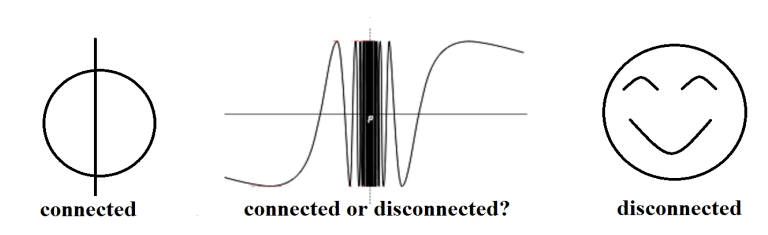
\includegraphics[width=0.6\textwidth]{figure/connectedness.png}
    \caption{}
\end{figure}

So we need a rigorous definition of connectedness (via the collection of open sets).
Before we give such a rigorous definition, let’s first look at a couple sets in $\R$
\begin{align*}
    (a)\  (0,3)\ (b)\ (0,1)\cup [2,3)\ (c)\ (0,1)\cup (1,3]\ (d)\ (0,1]\cup (1,3)
\end{align*}
Of course $(a)$ is connected, 
$(b)$ and $(c)$ are disconnected, 
while $(d)$ is connected! 
Although $(d)$ looks like a union of two intervals, they are really one interval $(0, 3)$ written
as a disjoint union of two subsets. The two subsets (0, 1] and (1, 3) are “attached”
together at the point 1, which is an element of (0, 1], but sits inside the closure of
(1, 3]. For the case (c), although the two “components” (0, 1) and (1, 3] sit “next to
each other”, it is still disconnected because (0, 1) contains no element in the closure of
(1, 3], and (1, 3] contains no element in the closure of (0, 1).
This example motivates us to define connectedness. Unlike most other conceptions
that you learned, connectedness is defined by its opposite. 

\section{Connectedness: The definition}
\begin{definition}{}{}
    Let $(X,\tau)$ be  topological space.\\
    (1) We say $X$ is disconnected, if there exists non-empty sets $A,B\subset X$ such that 
    \begin{align*}
        X=A\cup B \text{ and } A\cap \overline{B}=\overline{A}\cap B=\O.
    \end{align*}    
    (2) We say $X$ is connected if it is not disconnected.\\
    (3) We say a subset $X$ is connected/disconnected if it is connected/disconnected with respect to the subspace topology.
\end{definition}
\begin{remark}
    Note that by definition, the empty set is connected!
\end{remark}
\begin{remark}
    Suppose $A\subset X$ be a subset, then we say $A$ is connected if, 
    when endowed with the subspace topology, $(A,\tau_A)$ is connected. 
\end{remark}

\begin{proposition}{}{}
    Let $X$ be a topological space.
    Let $A\subset B\subset X$.
    Then $A$ is connected in B iff $A$ is connected in $X$.
\end{proposition}

\begin{proof}
    Let $\tau_A$ be the subspace topology on $A$ induced by $\tau$.
    Let $\tau_A'$be the subspace topology on $A$ induced by $\tau_B$.
    Then $A$ is connected in $X$ iff $(A,\tau_A)$ is connected.
    Similarly, $A$ is connected in $B$ iff $(A,\tau_A')$ is connected.
    By proposition\ref{prop:Subspace of Subspace is Subspace}, $\tau_A=\tau_A'$.
    Hence, $A$ is connected in $X$ iff $A$ is connected in $B$.
\end{proof}

\section{Connectedness: Equivalent characterizations.}

The definition above is intuitive but is also a little bit complicated. Fortunately
we have several other equivalent ways to describe connectedness.


\begin{proposition}{}{}
    For a topological space $X$, the following are equivalent:\\
    (1) $X$ is disconnected;\\
    (2) there exists non-empty disjoint open sets $A,B\subset X$ s.t. $X=A\cup B$;\\
    (3) there exists non-empty disjoint closed sets $A,B\subset X$ s.t. $X=A\cup B$;\\
    (4) there exists $A\neq \O$, $A\neq X$ such that $A$ is both open and closed in $X$.
\end{proposition}

\begin{proof}
    $(2)\Leftrightarrow (3)\Leftrightarrow (4)$ because
    \begin{align}
        A\cap B=\O \Leftrightarrow A^c=B, B^c=A.
    \end{align}
\end{proof}

\begin{proposition}{}{}
    For a topological space $X$, the following are equivalent:\\
    (1) $X$ is connected;\\
    (2) there is no non-empty disjoint open sets $A,B\subset X$ s.t. $X=A\cup B$;\\
    (3) $X$ and $\O$ are the only sets which are both open and closed in $X$.
\end{proposition}


\section{Examples of connected and disconnected spaces}
\begin{example}{}{}
    $(X,\tau_t)$ is connected, while $(X,\tau_s)$ is disconnected for $|X|\geqs 2$.
\end{example}

\begin{example}{}{}
    Infinite set with cofinite topology is connected.
\end{example}
\begin{proof}
    Let $(X,\tau_f)$ be an infinite set with cofinite topology. 
    Suppose $(X,\tau_f)$ is disconnected, then 
    $\exists$ non-empty open sets $A,B\subset X$ s.t. $A\cap B=\O$ and $X=A\cup B$.
    Then $X=\O^c=(A\cap B)^c=A^c\cup B^c$. Since $A,B$ is open in $(X,\tau_f)$, it follows that $A^c,B^c$ is finite and so $X$ is finite, 
    contradicting with the fact $X$ is infinite.
\end{proof}

\begin{example}
    Let $(X,\tau_c)$ be a co-countable topological space. 
    Show that $X$ is connected iff it is uncountable.
\end{example}
\begin{proof}
    ($\Leftarrow$):
    Suppose $(X,\tau_c)$ is disconnected when $X$ is uncountable, then 
    $\exists$ non-empty open sets $A,B\subset X$ s.t. $A\cap B=\O$ and $X=A\cup B$.
    Then $X=\O^c=(A\cap B)^c=A^c\cup B^c$. Since $A,B$ is open in $(X,\tau_c)$, 
    it follows that $A^c,B^c$ is countable and so $X$ is countable, 
    contradicting with the fact $X$ is uncountable.
\end{proof}


\begin{example}{}{}
    $\Q\subset \R$ is disconnected.
\end{example}

$\Q=((-\infty, -\sqrt{2})\cap \Q)\cup ((-\sqrt{2},+\infty)\cap \Q)$.

\begin{example}{}{}
    $S^1$(the unit circle in $\R^2$) is connected.
\end{example}

\begin{example}{}{}
    More generally, if $A \subset \R^2$ is countable, then $R^2 \setminus A$ is connected. 
    In particular, $R^2 \setminus Q^2$ is connected. 
    (Careful, this is not the set of all points with both coordinates irrational; it is
    the set of points such that at least one coordinate is irrational.)
\end{example}

\section{Connectedness in $\R$}

\begin{definition}{}{}
    A subset $S$ of $\R$ is said to be an interval if it has the following property: 
    if $x,z\in S$ and $y\in \R$ are such that $x<y<z$, then $y\in S$.
\end{definition}
\begin{remark}
    Each singleton set $\{x\}$ is an interval.
\end{remark}

\begin{remark}
    Every interval has one of the following forms: 
    $\{a\}$, $[a,b]$, $(a,b)$, $[a,b)$, $(a,b]$, $(-\infty,a)$, $(-\infty,a]$, $(a,\infty)$, $[a,\infty]$, $(-\infty,\infty)$.
\end{remark}

\begin{proposition}{}{}
    $\R$ is connected with respect to the euclidean topology.
\end{proposition}

\begin{proof}
    Suppose $\R$ is disconnected. Then there exists an open set 
\end{proof}

\begin{remark}
    By the same proof, one can show that all intervals
$(a, b)$, $[a, b]$, $(a, b]$, $[a, b)$,$(a,+\infty)$, $[a, +\infty)$,$(-\infty, b]$,
$(-\infty, b)$,$(-\infty, +\infty)$.
are connected.
\end{remark}









\section{Properties of connected spaces}
\subsection{Generalized intermediate value theorem}
\begin{proposition}{}{}
    Suppose $f:X\rightarrow Y$ is continuous. 
    Then for any connected subset $A\subset X$, 
    the image $f(A)\subset Y$ is connected.
\end{proposition}

\begin{proposition}{}{}
    A subspace of $R$ is connected if and only if it is an interval.
\end{proposition}

\begin{corollary}
    If $f:X\rightarrow Y$ is a homeomorphisom, then $X$ is connected iff $Y$ is connected.
\end{corollary}

\begin{corollary}{}{}
    If $X$ is connected, $f:X\rightarrow \R$ is continous, 
    and if there exist $x_1,x_2\in X$ s.t. $f(x_1)=a<b=f(x_2)$,
    then for any $a<c<b$, there exists $x\in X$ s.t. $f(x)=c$.
\end{corollary}

\subsection{The closure}

\begin{lemma}{}{connected subset with clopen subset}
    Let $X_0\subset X$ be both open and closed and $A\subset X$ be connected. 
    Then either $A\cap X_0=\O$ or $A\subset X_0$.
\end{lemma}

\begin{proof}
    If $X_0$ is both open and closed in $X$, then $A\cap X_0$ is both open and closed in $A$.
    Since $A$ is connected, it follows that the only sets which is both open and closed in $A$ is $A$ and $\O$.
    Then either $A\cap X_0=\O$ or $A\cap X_0=A$(implies $A\subset X_0$).
\end{proof}

\begin{proposition}{}{}
    If $X$ has a connected dense subset, then $X$ is connected.
\end{proposition}
\begin{proof}
    Suppose $A$ is a connected dense subset of $X$ and $X_0$ is a subset which is both open and closed.
    If $X_0\neq \O$, then $X_0\cap A\neq \O$, by lemma\ref{lem:connected subset with clopen subset}, $A\subset X_0$. 
    Then $X=\overline{A}\subset \overline{X_0}=X_0$. Then the only sets which is both open and closed in $X$ are $X$ and $\O$.
    Hence, $X$ is connected.
\end{proof}

\begin{corollary}{}{}
    Let $A$ be a connected subset of $X$. If $A\subset Y\subset \overline{A}$, then $Y$ is connected.
\end{corollary}
\begin{proof}
    Since $\text{cl}_Y(A)=Y\cap \text{cl}_X(A)=Y$, it follows that $A$ is a connected dense subset of $Y$ and so $Y$ is connected. 
\end{proof}

\begin{corollary}{}{}
    If $A$ is connected, so is $\overline{A}$.
\end{corollary}
\begin{proof}
    $A\subset \overline{A}\subset\overline{A}$.
\end{proof}

\begin{corollary}{Topologist's sine curve}{Topologist's sine curve is connected}
    The set 
    \begin{align*}
        S=\{(x,y):x\in (0,1),y=sin\frac{1}{x}\}\cup \{(0,y):y\in [-1,1]\}\subset \R^2
    \end{align*}
    is connected.
\end{corollary}

\subsection{The union}

\begin{proposition}{}{}
    Let $A_{\alpha}\subset X$ be a collection of non-empty connected subsets in $X$, 
    and assume $\cap_{\alpha}A_{\alpha}\neq \O$. Then $\cup_{\alpha}A_{\alpha}$ is connected. 
\end{proposition}
\begin{proof}
    Denote $Y=\cup_{\alpha}A_{\alpha}$. 
    Suppose $X_0$ is both open and closed in $Y$, we should show that $X_0=\O$ or $Y$.
    
\end{proof}

\section{The product}
\begin{proposition}{}{}
    If $X$, $Y$ are connected, so is $X \times Y$ .
\end{proposition}


\section{Locally connected}

\begin{definition}{}{}
    A topological space $X$ is locally connected at a point $x\in X$ if every neighbourhood $U$ of $x$ contains a connected neighbourhood $K$ of $x$.
    The space $X$ is locally connected if it is locally connected at every point $x\in X$.
\end{definition}


\section{Exercise}

\begin{exercise}{}{}
    Open subset of locally connected space is locally connected.
\end{exercise}

% \begin{proof}
%     Suppose $X$ is locally connected and $A\subset X$ is open. 
%     To show that $(A,\tau_A)$ is a locally connected topological space, 
%     we must prove that every neighbourhood $U$ of $x\in A$ contains connected elements of $\tau_A$, which implies $U$ contains a connected neighbourhood of $x$.
%     Since $X$ is locally connected, there exists $\tilde{\mathcal{B}}=\{O_{\alpha}\in \tau:\alpha\in I\}$ 
%     in which $O_{\alpha}$ is connected and $O_{\alpha}$ contains $x$ such that $x\in O_{\alpha}\subset U$ for some $\alpha\in I$.
%     Let $\mathcal{B}=\{O_{\alpha}\cap A:\alpha\in I\}$. We claim that $\mathcal{B}$ is a neighbourhood basis of $x$ in $A$.
%     In fact, Let $N\in \tau_A$ such that $x\in N$, then $\exists K\in \tau$ such that $N=K\cap A$. Then $N\in \tau$ as $K,A\in \tau$.
%     Then one can find $\alpha\in I$ such that $x\in O_{\alpha}\subset N$. Then $O_{\alpha}\cap A\subset N\cap A$. 
%     Since $N\subset A$, it follows that $O_{\alpha}\cap A\subset N$ as required. 
%     Now we use $\mathcal{B}$ to construct a connected neighbourhood basis of $x$.
%     Define $\phi:\mathcal{B}\rightarrow I$ such that $O_{\phi(N)}\subset N$. 
%     $O_{\phi(N)}\in \tau$ and $O_{\phi(N)}\subset N\subset A$. Then $O_{\phi(N)}=O_{\phi(N)}\cap A\in \tau_A$.
%     Since $O_{\phi(N)}$ is connected in $X$ and $O_{\phi(N)}\subset A$. Then $O_{\phi(N)}$ is connected in $A$.
%     Then for any $V\in\tau_A$ such that $x\in V$, there exist $N\in \mathcal{B}$ such that $x\in O_{\phi(N)}\subset N\subset V$
% \end{proof}

\begin{proof}
    Suppose $(X,\tau)$ is locally connected and $A\subset X$ is open. 
    For $x\in A$ and any neighbourhood $N$ of $x$ in $A$, $\exists U\in \tau_A$ such that $x\in U\subset N\subset A$.
    Then $U=O\cap A$ where $O\in \tau$. Then $U\in \tau$. Then $N$ is neighbourhood of $x$ in $X$.
    Since $X$ is locally connected, it follows that there exists connected neighbourhood $K$ of $x$ in $X$ and $V\in\tau$ such that 
    $x\in V\subset K\subset N\subset A\subset X$. 
    Then $K$ is connected in $A$ and $V=V\cap A\in\tau_A$. 
    Hence, K is a connected neighbourhood of $x$ in $A$.
    and so $A$ is locally connected.
\end{proof}

\begin{exercise}{P66 T7}{}
    $X$ is disconnected $\Leftrightarrow$ there exists a continuous function $f:X\rightarrow E^1$
    such that $f(X)$ only has two points.
\end{exercise}

\begin{proof}
    ($\Rightarrow$): If $X$ is disconnected, then there exists non-empty open sets $U,V$ s.t. 
    $X=U\cup V$ and $U\cap V=\O$. Define $f:X\rightarrow E^1$ such that $f(U)=0$ and $f(V)=1$.
    We claim that $f$ is continuous. For any open set $W$ in $E^1$, 
    if $0,1$ are not in $W$, then $f^{-1}(W)=\O$, which is open. If $0\in W$, $f^{-1}(W)=U$ which is open. 
    If $1\in W$, then $f^{-1}(W)=V$ which is open. Hence, $f$ is continous.
    \\
    ($\Leftarrow$): Suppose $X$ is connected. Since $f$ is continous, it follows that $f(X)$ is connected.
    But $f(X)=\{a,b\}$ ($a,b\in E^1$) is disconnected. 
\end{proof}

\begin{exercise}{P66 T8}{}
    Let $X$ be a subset of $E^2$ and $X=\{(x,y): \text{ not all } x,y \text{ are irrational} \}$.
    Then $X$ is connected.  
\end{exercise}

\begin{proof}
    $\forall r\in \Q$, let $A_r=\{(x,y):\text{either }x \text{ or } y \text{ is rational}\}$. 
    Let $A=E^1\times \{r\}$ and $B=\{r\}\times E^1$, then $A,B$ are connected and $A_r=A\cup B$, $A\cap \{(r,r)\}\neq \O$ and $B\cap \{(r,r)\}\neq \O$. 
    Hence, $A_r$ is connected. Since $X=\cup_{r\in \Q} A_r$ and $A_r\cap A_0\neq \O$, it follows that $X$ is connected.
\end{proof}


\section{Reference}

\begin{itemize}
    \item \href{https://ece.iisc.ac.in/~parimal/2015/proofs/lecture-18.pdf}{Lecture 18: Connectedness}
    \item \href{https://www.math.toronto.edu/ivan/mat327/docs/notes/18-connected.pdf}{18. Connectedness}
    \item \href{http://staff.ustc.edu.cn/~wangzuoq/Courses/21S-Topology/Notes/Lec16.pdf}{CONNECTEDNESS}
\end{itemize}
\chapter{Path Connectedness}\label{chp:2_5}


\chapter{Topological Properties and Homeomorphism}\label{chp:2_6}

\begin{proposition}{}{}
    If $a,b,c,d$ are any real numbers with $a<b$ and $c<d$, then
    \begin{align*}
        (0,1)\cong (a,b)\cong (c,d)\cong \R.
    \end{align*}
\end{proposition}

\begin{proposition}{}{}
    If $a,b,c,d$ are any real numbers with $a<b$ and $c<d$, then
    \begin{align*}
        [a,b]\cong [c,d].
    \end{align*}
\end{proposition}

\begin{proposition}{}{}
    If $a,b$ are any real numbers, then 
    \begin{align*}
        (-\infty,a]\cong (-\infty, b] \cong [a,\infty) \cong [b,\infty).
    \end{align*}
\end{proposition}

\begin{proposition}{}{}
    If $c,d,e$ and $f$ are any real numbers with $c<d$ and $e<f$, then 
    \begin{align*}
        [c,d)\cong [e,f)\cong (c,d]\cong (e,f].
    \end{align*}
\end{proposition}

\begin{proposition}{}{}
    If $a,b$ are any real numbers, then 
    \begin{align*}
        [0,1)\cong (-\infty,a]\cong  [a,\infty) \cong [a,b)\cong (a,b].
    \end{align*}
\end{proposition}


\begin{proposition}{}{}
    Let $f:(X,\tau)\rightarrow (Y,\tau')$ be a homeomorphism. Let $a\in X$, 
    so that $X\setminus\{a\}$ is a subspace of $X$ and has induced topology $\tau_1$.
    Also $Y\setminus \{f(a)\}$ is subspace of $Y$ and has induced topology $\tau_1'$. 
    Then $(X\setminus \{a\},\tau_1)$ is homeomorphic to $(Y\setminus \{f(a)\},\tau_1')$.
\end{proposition}



\begin{proof}
    Suppose $f:X\rightarrow Y$ is a homeomorphism. 
    Define $g:X\setminus \{a\} \rightarrow Y\setminus\{f(a)\}$. 
    Since $f$ is bijection, it follows that $g$ is bijection.
    For open set $U$ in $(X\setminus \{a\},\tau_1)$, then $\exists O\in \tau$ such that $U=O\cap (X\setminus \{a\})$.
    Then $g(U)=f(O\cap (X\setminus \{a\}))\overset{f \text{ is injective }}{=} f(O)\cap (Y\setminus \{f(a)\})\in \tau_1'$.
    For open set $K$ in $(Y\setminus \{f(a)\},\tau_1')$, then $\exists V \in \tau'$ such that $K=V\cap (Y\setminus \{f(a)\})$
    Then $g^{-1}(K)=f^{-1}(V\cap (Y\setminus \{f(a)\}))=f^{-1}(V)\cap (X\setminus \{a\})\in\tau_1$.
\end{proof}

\begin{proposition}{}{}
    Any topological space homeomorphic to a connected space is connected.
\end{proposition}


This proposition gives us one way to show two topological spaces are not homeomorphic, 
by finding a property "preserved by homeomorphisms" which one space has and the other does not.
We have met many properties "preserved by homeomorphisms":
\begin{itemize}
    \item $T_1$
    \item $T_2$
    \item $T_3$
    \item $T_4$
    \item separable
    \item $C_1$
    \item $C_2$
    \item connected
    \item locally connected
    \item path-connected
    \item locally path-connected
    \item compact
    \item sequentially compact
\end{itemize}

\begin{corollary}{}{}
    If $a,b,c$ and $d$ are real numbers with $a<b$ and $c<d$, then\\
    (1) $(a,b)\not\cong [c,d)$,\\
    (2) $(a,b)\not\cong [c,d]$,\\
    (3) $[a,b)\not\cong [c,d]$.
\end{corollary}

\begin{proof}
    (1) If $(a,b)\cong [c,d)$, then $(a,b)\setminus \{x\} \cong (c,d)$, but $(a,b)\setminus \{x\}$ is disconnected and $(c,d)$ is connected.
\end{proof}

\begin{theorem}{}{}
    Let $X$ be compact and $Y$ be Hausdorff space. 
    If $f:X\rightarrow Y$ is continous and bijective, then
    $f$ is homeomorphism.
\end{theorem}

\begin{definition}{}{}
    $E^1:=\R$, $E^2:=\R^2$,$E^n:=\R^n$\\
    $S^1:=\{(x,y)\in E^2:x^2+y^2=1\}$, $S^2:=\{(x,y,z)\in E^3:x^2+y^2+z^2=1\}$\\
    $S^{n-1}=\{(x_1,...,x_n)\in E^n:\sum\limits_{i=1}^{n}x_i^2=1\}$\\
    $D^n=\{x\in E^n:||x||\leqs 1\}$ where $||x||$ is the distance from $x$ to origin.
\end{definition}

\begin{proposition}{}{}
    \text{Int}($D^n$)$\cong$ $E^n$.
\end{proposition}

\begin{proposition}{}{}
    $S^n\setminus \{N\}\cong E^n$ ($N$ is the north point of $S^n$).
\end{proposition}

\begin{proposition}{}{}
    $E^n\setminus \{O\}\cong E^n\setminus D^n$ ($O$ is origin).
\end{proposition}

\begin{proof}
    $f:E^n\setminus \{O\}\rightarrow E^n\setminus D^n$ given by $f(x)=x+\frac{x}{||x||}$
\end{proof}

\begin{proposition}{}{}
    $E^n\setminus \{O\}\cong S^{n-1}\times E^1$. 
\end{proposition}
    $\R^+\cong \R\Rightarrow S^{n-1}\times \R^+\cong S^{n-1}\times \R$\\
    $f:\R^n\setminus \{O\}\rightarrow S^{n-1}\times \R^+$ given by $f(x)=(\frac{x}{||x||},||x||)$


\begin{proposition}{}{}
    $E^1\not\cong E^n$ ($n>1$).
\end{proposition}
    $E^1\setminus \{O\}$ is not connected.\\
    $E^n\setminus \{O\}\cong S^{n-1}\times E^1$ is connected. 
\begin{proposition}{}{}
    $I\not\cong S^1$.
\end{proposition}
   For $x\in \text{Int}(I)$, $I\setminus \{x\}$ is not connected.
   $S^1\setminus \{f(x)\}\cong E^2$ is connected.

\begin{proposition}{}{}
    $S^2\not\cong S^1$.
\end{proposition}
    $S^2\setminus \{N_2\}\cong E^2$, $S_1\setminus \{N_1\}\cong E^1$, but $E^1\not\cong E^2$.

\begin{proposition}
    If $f:S^1\rightarrow E^1$ is continuous, then $f$ is not injective and surjective.
\end{proposition}


\begin{proposition}{}{}
    
\end{proposition}

\section{Reference}

\begin{itemize}
    \item \href{}{topology without tears chp4}
\end{itemize}


\part{}
\chapter{Quotient Space and Quotient Mapping}\label{chp:3_2}


We have seen how to create new topological spaces from given topological spaces
using the operation of forming a subspace and the operation of forming a product of a set of topological spaces.
In this chapter we introduce a third operation, namely that of forming a quotient space(of a topological space).
As examples we shall see the Klein bottle and M\"obius strip.

\section{Quotient spaces}

\begin{definition}{}{}
    Let ($X$,$\tau$) be a topological space and let $X^*$ be a partition of $X$ into
    disjoint subsets whose union is $X$. Let $p:X$ → $X^*$ be the surjective (onto) map
    that carries each point of $X$ to the element of $X^*$
    containing it. $p$ is called the
    projection map from $X$ to $X^*$
    . In the topology on $X^*$
    induced by $p$ ($\tau^*=\{U\subset X^*: p^{-1}(U)\in\tau\}$), the space $X^*$ under this topology is the quotient space of $X$.
\end{definition}

Note. Recall that we have a partition of a set if and only if we have an equivalence
relation on the set. So the approach in terms
of partitions can be replaced with an approach based on equivalence relations.
The idea of the quotient space is that points of the subsets in the partition (or
the equivalent points under the equivalence relation) are “identified” with each
other. For this reason, quotient spaces are sometimes called “identifying spaces” or
“decomposition spaces.” You will notice the parallel between quotient spaces and
quotient groups in which all elements of a coset are identified.

Then we can get the definition of quotient space by the equivalence relation.

\begin{definition}{}{}
    Let ($X$,$\tau$) be a topological space and and $\sim$ any equivalence relation on $X$.
    Let $X/\sim$ be the set of all equivalence classes of $\sim$ and $p:X$ → $X/\sim$ given by $x\mapsto [x]$. 
    In the topology on $X/\sim$
    induced by $p$ ($\tilde{\tau}=\{U\subset X/\sim: p^{-1}(U)\in\tau\}$), the space $X/\sim$ under this topology is the quotient space of $X$.
\end{definition}

\begin{definition}{}{}
    Let $(X,\tau)$ and $(Y,\tau_1)$ be topological spaces.
    Then $(Y,\tau_1)$ is said to be a quotient space of $(X,\tau)$ if there exists a mapping $f:(X,\tau)\rightarrow (Y,\tau_1)$ satisfying the following properties: \\
    (1) $f$ is surjective.\\
    (2) For each subset $U$ of $Y$, $U\in \tau_1\Leftrightarrow f^{-1}(U)\in \tau$.
    And $f$ is said to be a quotient mapping.
\end{definition}

\begin{remark}
    From the definition, it is clear that every quotient mapping is continous.
\end{remark}

\begin{remark}
    Property (2) is equivalent to: For each subset $A$ of $Y$, 
    $A$ is closed in $(Y,\tau_1)\Leftrightarrow f^{-1}(A)$ is closed in $(X,\tau)$.
\end{remark}

\begin{proposition}{}{}
    If $f:(X,\tau)\rightarrow (Y,\tau_1)$ is a surjective, continous and open mapping, then $f$ is a quotient mapping.
    If $f$ is a surjective, continous and closed mapping, then it is a quotient mapping.
\end{proposition}
\begin{proof}
    If $f$ is continous and surjective, then (1) and necessary condition of (2) hold.
    If $f$ is open, then if $f^{-1}(U)\in \tau$ ,then $U=f(f^{-1}(U))\tau$. 
\end{proof}

\begin{proposition}{}{}
    $f:(X,\tau)\rightarrow (Y,\tau_1)$ is injective. Then $f$ is a homeomorphism iff it is a quotient mapping.
\end{proposition}
\begin{proof}
    ($\Rightarrow$): $f$ is homeomorphism, then $f$ is continous and surjective.
    And for $U\in Y$, if $f^{-1}(U)\in \tau$, then $U=f(f^{-1}(U))\in \tau_1$.
    \\
    ($\Leftarrow$): $f$ is quotient mapping then $f$ is continous and surjective. Then $f$ has an inverse $f^{-1}$.
    For $K\in \tau$, $K=f^{-1}(f(K))\in\tau$ as $f$ is bijective. Then, $f(K)\in \tau_1$. Hence, $f^{-1}$ is continous.
\end{proof}

\begin{proposition}{}{}
    Let $X$ be compact and $Y$ be Hausdorff space. If $f:X\rightarrow Y$ is continous and surjective, then
    $f$ is a quotient mapping.
\end{proposition}

\begin{proof}
    Let $A$ be a closed set in $X$. Since $X$ is compact, it follows that $A$ is compact. 
    Then $f(A)$ is compact as $f$ is continous. Since $Y$ is Hausdorff, it follows that $f(A)$ is closed.
    Then $f$ is continous, surjective and closed mapping. Hence, $f$ is a quotient mapping. 
\end{proof}

\begin{proposition}{Universality}{}
    Let $f:X\rightarrow X'$ be a quotient mapping and 
    $g:X'\rightarrow Y$ be a map. Then $g$ is continous iff $g\circ f$ is continous.
\end{proposition}

\begin{proof}
    ($\Rightarrow$): $f$ is a quotient mapping, then $f$ is continous. Then $g\circ f$ is continous as $g$ is continous.
    \\
    ($\Leftarrow$): For open set $U$ in $Y$, then $(gf)^{-1}(U)=f^{-1}(g^{-1}(U))$ is open in $X$.
    Then $g^{-1}(U)$ is open in $X'$ as $f$ is a quotient mapping. Hence, $g$ is continous. 
\end{proof}

Let $f:X\rightarrow Y$ be a mapping, we define a equivalence relation $\overset{f}{\sim}$:
$\forall x,x'\in X, x\sim x'\Leftrightarrow f(x)=f(x')$.

\begin{proposition}{}{}
    If $f:X\rightarrow Y$ is a quotient mapping, then $X/\overset{f}{\sim}\cong Y$.
\end{proposition}




\section{Exercise}

\begin{exercise}{P86 T1}{}
    Let $f:X\rightarrow Y$ and $g:Y\rightarrow Z$ be continuous mapping such that $g\circ f$ is a quotient mapping. 
    Then $g$ is quotient mapping.
\end{exercise}

\begin{proof}
    Since $g\circ f$ is a quotient mapping, it follows that $g\circ f$ is surjective and 
    for $U\subset Z$, $U$ is open in $Z$ $\Leftrightarrow$ $f^{-1}(g^{-1}(U)$) is open in $X$.
    Then for any $z\in Z$, $\exists x\in X$ such that $z=g(f(x))$. Let $y=f(x)$, then $y\in Y$ and $z=g(y)$.
    Hence, $g$ is surjective. If $U$ is open in $Z$, then $g^{-1}(U)$ is open in $Y$ as $g$ is continous.
    If $g^{-1}(U)$ is open in $Y$, then $f^{-1}(g^{-1}(U))$ is open in $X$ as $f$ is continous, then $U$ is open in $Z$.
    Hence, $g$ is a quotient mapping.
\end{proof}

\begin{exercise}{P86 T2}{}
    Let $f:X\rightarrow Y$ be a quotient mapping , $B$ be open(or closed) set of $Y$
    and $A=f^{-1}(B)$. Then $f_A:A\rightarrow B$ is a quotient mapping.
\end{exercise}

\begin{proof}
    Since $f$ is a quotient mapping, it follows that $f$ is surjective and for $U\subset Y$, $U$ is open in $Y$ $\Leftrightarrow$ $f^{-1}(U)$ is open in $X$.
    Then $A=f^{-1}(B)$ is open in $X$ as $B$ is open in $Y$ and $f$ is continous.
    Since $f$ is surjective, it follows that $f_A(A)=f(A)=f(f^{-1})(B)=B$. Then $f_A$ is surjective.
    For $K\subset B$, if $K$ is open in $B$, then $K=O_Y\cap B$ ($O_Y$ is open in $Y$) is open in $Y$, then $f_A^{-1}(K)=f^{-1}(K)\subset A$ is open in $X$ , then $f_A^{-1}(K)=f_A^{-1}(K)\cap A$ and so open in $A$.
    If $f_A^{-1}(K)$ is open in $A$, then $f^{-1}(K)=f_A^{-1}(K)=O_X\cap A$ ($O_X$ is open in $X$) is open in $X$, then $K\subset B$ is open in $Y$, then $K=K\cap B$ and so open in $B$. 
    Hence, $f_A$ is a quotient mapping.
\end{proof}

\section{Reference}

\begin{itemize}
    \item \href{http://staff.ustc.edu.cn/~wangzuoq/Courses/21S-Topology/Notes/Lec06.pdf}{THE QUOTIENT TOPOLOGY}
    \item \href{}{topology without tears ch11}
\end{itemize}


\chapter{Homotopies}\label{chp:4_1}

Recall that a path is a continuous function $a : [0, 1] \rightarrow X$. 
The idea here is that we have two paths $a_0$ and $a_1$ in $R^2$ 
with $a_0(0) = a_1(0)$ and $a_0(1) = a_1(1)$;
i.e. the paths have the same endpoints.

\begin{figure}[H]
    \centering
    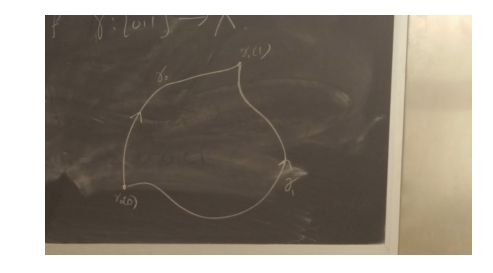
\includegraphics[width=0.6\textwidth]{figure/homotopy1.png}
    \caption{}
\end{figure}

Our paths are different and may even have different images, but we want to say that one
can be continuously deformed into the other.

\begin{figure}[H]
    \centering
    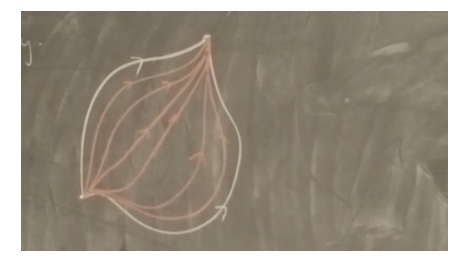
\includegraphics[width=0.6\textwidth]{figure/homotopy2.png}
    \caption{}
\end{figure}

Intuitively, we want to create a family of paths $\{a_t\}_{t\in[0,1]}$ “from $a_0$ to $a_1$.” 
You can also say we want to interpolate continuously between $a_0$ and $a_1$. 
Think of $\{a_t: t \in [0, 1]\}$
as one function $a : [0, 1] \times [0, 1] \rightarrow X$, 
where $a(x, t) := a_t(x)$.


The notion $C(X,Y)$ is the set of all the continuous maps from $X$ to $Y$.

Two continuous functions from one topological space to another are called homotopic if one can be “continuously deformed” into the other, such a deformation being
called a homotopy between the two functions. More precisely, we have the following
definition.

\begin{definition}{}{}
    Let $X, Y$ be topological spaces, and $f, g : X \rightarrow Y$ continuous maps.
A homotopy from $f$ to $g$ (denoted by $H: f\simeq g$) is a continuous function $H : X \times [0, 1] \rightarrow Y$ satisfying
$H(x, 0) = f(x)$ and $H(x, 1) = g(x)$, for all $x \in X$.
If such a homotopy exists, we say that $f$ is homotopic to $g$, 
and denote this by $f\simeq g:X\rightarrow Y$ or $f\simeq g$. 
\end{definition}

\begin{definition}{}{}
    If $f$ is homotopic to a constant map, i.e., if $f \simeq \text{const}_y$, 
for some $y \in Y$ , then we say that $f$ is nullhomotopic.
\end{definition}

\begin{proposition}{}{}
    Let $f, g : E^n \rightarrow E^n$ any two continuous, real functions. 
    Then $f \simeq g$. 
\end{proposition}
To see why this is the case, 
define a function $F : E^n \times [0, 1] \rightarrow E^n$ by
$H(x,t)=(1-t)\cdot f(x)+t\cdot g(x)$.
$H$ is continuous and $H(x,0)=f(x),H(x,1)=g(x)$. 
Thus, $H$ is a homotopy between $f$ and $g$.

\begin{proposition}{}{}
    Let $A$ be a convex subset of $E^n$, endowed with the subspace topology,
and let $X$ be any topological space. Then any two continuous maps $f, g : X \rightarrow A$ are
homotopic. The homotopy from $f$ to $g$ called the straight line homotopy.
\end{proposition}

\begin{proposition}{}{}
    If $Y$ is convex, $p \in Y$ , $f : X \rightarrow Y$ 
    is continuous, and $g : X \rightarrow Y$ is $g(x) = p$
    for all $x \in X$, then $f \simeq g$ via the straight line homotopy.
\end{proposition}



\begin{proposition}{}{}
    Homotopy is an equivalence relation on $C(X, Y)$.
\end{proposition}

\begin{proposition}{}{}
    If $f_0\simeq f_1: X\rightarrow Y$,
    $g_0\simeq g_1:Y\rightarrow Z$, then
    $g_0\circ f_0\simeq g_1\circ f_1:X\rightarrow Z$.
\end{proposition}

\begin{proposition}{}{}
    Let $y_1,y_2\in Y$ and $f_{y_i}:X\rightarrow Y$ given by $f(X)=y_i$.
    Then $f_{y_1}\simeq f_{y_2}\Leftrightarrow$ $y_1$ and $y_2$ is in the same path component.
\end{proposition}


\begin{proposition}{}{}
    If $Y$ is path-connected, then the set $[I,Y]$ 
    (the homotopy classes of maps from $I$ to $Y$) 
    has a single element.
\end{proposition}


For our paths, we want to fix the start and end, so $a_t(0) = a_t(1) = a_0(1)$ for all $t \in [0, 1]$.

\begin{definition}{}{}
    Let $A\subseteq X$ and $f,g\in C(X,Y)$.
    We say $f$ and $g$ are homotopic relative to $A$ iff there exists a homotopy $H$ between $f$ and $g$, and:\\
    (1) $\forall a\in A$: $f(a)=g(a)$\\
    (2) $\forall a\in A, t\in [0,1]$: $H(a,t)=f(a)$\\
    and denote this by $f\simeq g \text{ rel}A$ and $H:f\simeq g\text{ rel}A$.
\end{definition}

\begin{proposition}{}{}
    If $A\subseteq X$, homotopy relative to $A$ is an equivalence relation on $C(X, Y)$.
\end{proposition}

\begin{proposition}{}{}
    If $f_0\simeq f_1: X\rightarrow Y \text{ rel}A$,
    $g_0\simeq g_1:Y\rightarrow Z\text{ rel}B$ and $f_0(A)\subset B$, then
    $g_0\circ f_0\simeq g_1\circ f_1 \text{ rel}A$.
\end{proposition}

\begin{definition}{}{}
    Let $a$ and $b$ be paths in $X$. $a$ is path-homotopic to $b$ if $a\simeq b \text{ rel}\{0,1\}$
    and denoted by $a \underset{\cdot}{\simeq} b$. i.e.
    there exists a homotopy $H$ between $a$ and $b$ such that:\\
    (1) $a(0)=b(0),a(1)=b(1)$\\
    (2) $\forall t\in [0,1]$: $H(0,t)=a(0), H(1,t)=a(1)$.
\end{definition}

\begin{figure}[H]
    \centering
    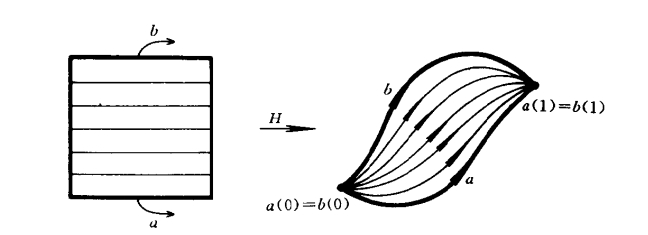
\includegraphics[width=0.6\textwidth]{figure/path-homotopic.png}
    \caption{}
\end{figure}

Since homotopy relative to a subset is an equivalence relation, 
it follows that path-homotopy is a equivalence relation on the set $P(X)$ of all paths in $X$.
Then path-homotopy be a partition of $P(X)$ into
disjoint subsets whose union is $P(X)$. These disjoint subsets are called path classes in $X$.
The collection of all path classes is denoted by $[X]$.
Given path $a$, the path classes $a$ belongs to denoted by $<a>$.
The startpoint and endpoint of $a$ are the startpoint and endpoint of $<a>$.
The path class is call closed path class if its startpoint and endpoint coincide, 
then its startpoint(endpoint) is called base point.


\section{Reference}
\begin{itemize}
    \item \href{https://www.math.toronto.edu/~herzig/MAT327-lecturenotes21b.pdf}{Path Homotopy}
    \item \href{https://www.ms.uky.edu/~guillou/F17/551Notes-Week15.pdf}{Path-homotopy}
    \item \href{http://staff.ustc.edu.cn/~wangzuoq/Courses/21S-Topology/Notes/Lec18.pdf}{HOMOTOPY AND PATH HOMOTOPY}
    \item \href{https://pillowmath.github.io/Math%20142/Lec9.pdf}{Homotopy}
\end{itemize}
\chapter{Fundamental Group}\label{chp:4_2}

\section{Reference}

\begin{itemize}
    \item \href{https://pillowmath.github.io/Math%20142/Lec10.pdf}{The Fundamental Group}
    \item \href{https://www.ms.uky.edu/~guillou/F17/551Notes-Week15.pdf}{The fundamental group}
\end{itemize}
\chapter{The Fundamental Group of $S^n$}\label{chp:4_3}


\begin{proposition}{}{}
    $\pi_1(S_1)\cong\Z$.
\end{proposition}

\begin{proposition}{}{}
    Let $X, Y$ be path-connected. Then $\pi_1(X \times Y )$ is isomorphic to $\pi_1(X) \times \pi_1(Y)$.
\end{proposition}

\begin{proposition}{}{}
    $\pi_1(S^n) = \{0\}$ for $n > 2$.
\end{proposition}

\begin{proposition}{}{}
    $T^2\not\cong S^2$.
\end{proposition}
\begin{proof}
    $\pi_(S^1)\cong \Z$, $T^2=S^1\times S^1$, then $\pi_1(T^2)\cong \Z\times \Z$, but $\pi_1(S^2)=\{0\}$.
\end{proof}

\section{Reference}

\begin{itemize}
    \item \href{https://www.math.toronto.edu/mgualt/MAT1300/Week%202%20Term%202.pdf}{$\pi_1(S^1)\cong Z$}
\end{itemize}

\chapter{Exam Exercise1}

\begin{exercise}{}{}
    $X=\{a,b,c,d\}$, $\tau=\{X,\O,\{a\}\}$, then $\overline{\{b\}}=$?
\end{exercise}

\begin{proof}
    To  find the closure of a particular set, we shall find all the closed set containing that set and then select the smallest.
    The closed sets in $X$ are $\O,X,\{b,c,d\}$.
    Then, $\overline{\{b\}}=\{b,c,d\}$.
\end{proof}

\begin{exercise}{}{}
    $X=\{a,b,c,d\}$, $\tau={X,\O,\{a\},\{b,c,d\}}$, 
    the number of proper subsets of $X$ which are both open and closed is ?
\end{exercise}

\begin{proof}
    The closed sets of $X$ are $X,\O,\{b,c,d\},\{a\}$.
    Then the proper subsets of $X$ which are both open and closed are $\{b,c,d\},\{a\}$.
\end{proof}

\begin{exercise}{}{}
    In $\R$, $\Q^{\circ}(\text{Int}(\Q))=$?
\end{exercise}

\begin{proof}
    $\Q^{\circ}=\O$.
    The interior of set in topological space 
    is the largest open set contained in the set. 
    In the euclidean topology, 
    there is no non-empty open interval contained entirely in $\Q$.
    since between any two rational numbers, there is an irrational number.
\end{proof}

\begin{exercise}{}{}
    In $\R$, $\partial(\Q)=$?
\end{exercise}

\begin{proof}
    $\partial(\Q)=\R$. 
    Since $\partial(A)=\overline{A}\setminus \text{Int}(A)$ and $\overline{Q}=\R$,
    it follows that $\partial(\Q)=\R\setminus \O=\R$.
\end{proof}

\begin{exercise}{}{}
    In $\R$, $\Z^{\circ}(\text{Int}(\Z))=$?
\end{exercise}

\begin{proof}
    $\Z^{\circ}=\O$.
    The interior of set in topological space 
    is the largest open set contained in the set. 
    In the euclidean topology, 
    there is no non-empty open interval contained entirely in $\Z$.
    since between any two rational numbers, there is an irrational number.
\end{proof}

\begin{exercise}{}{}
    In $\R$, $\partial(\Z)=$?
\end{exercise}

\begin{proof}
    $\overline{\Z}=\Z$. $\Z$ is closed since $\Z=\R\setminus(\cup_{n\in \R}(n,n+1))$.
\end{proof}

\begin{exercise}{}{}
    (1) $(A\cup B)'=A'\cup B'$\\
    (2) $\overline{A\cup B}=\overline{A}\cup \overline{B}$
\end{exercise}

\begin{exercise}{}{}
    Let $X$ be a discret space and $A\subset X$, then $A'=$?
\end{exercise}
\begin{proof}
    $A'=\O$. For every $x\in X$, $x\in \{x\}$ which is open,$\{x\}\cap A\setminus\{x\}=\O$.
\end{proof}

\begin{exercise}{}{}
    Let $X$ be a trival space and $A\subset X$. Then\\
    (1) $A=\O$,then $A'=\O$\\
    (2) If $A=\{x_0\}$, then $A'=X\setminus A$\\
    (3) If $A=\{x_1,x_2\}$, then $A'=X$.
\end{exercise}

\begin{proof}
    (1) If $A=\O$, $\O\subset X$ but $X\cap A\setminus \O=\O$.\\
    (2) For $x\in X\setminus A$, $x\in X$ which is open, $X\cap A\setminus\{x\}=\{x_0\}$.
    If $x\in A$, then $X\cap A\setminus \{x\}=\O$.\\
    (3) For $x\in X\setminus A$, $x\in X$ which is open, $X\cap A\setminus\{x\}=\{x_1,x_2\}$.
    If $x\in A$, then $X\cap A\setminus \{x\}=\{x_1\}$ or $\{x_2\}$.
\end{proof}

\begin{exercise}{}{}
    $X=\{a,b,c,d\}$, $B=\{\{a,b,c\},\{c\},\{d\}\}$,
    then the topology induced by $\mathcal{B}$ is $\{X,\O,\{c\},\{d\},\{c,d\},\{a,b,c\}\}$.
\end{exercise}

\begin{proof}
    Let $(X,\tau)$ be a topological space. 
    A collection $\mathcal{B}$ of subsets of $X$ is said to be a basis for the topology $\tau$
    if $\ob=\tau$.
\end{proof}

\begin{exercise}{}{}
    Any subset of discret space is both open and closed.
\end{exercise}
\begin{proof}
    
\end{proof}

\begin{exercise}{}{}
    Any subset of trival space is neither open nor closed.
\end{exercise}

\begin{exercise}{}{}
    Any singleton of $\R$ is closed.
\end{exercise}

\begin{proof}
    $\R\setminus \{x\}=\cup_{a,b\in \R\setminus \{x\}}(a,b)\cup (x,x+1)\cup (x-1,x)$ is open.
\end{proof}

\begin{exercise}{}{}
    In $\R$, $A=\{1,\frac{1}{2},\frac{1}{3},...\}$, then $\overline{A}=$?
\end{exercise}

\begin{proof}
    $\overline{A}=A\cup \{0\}$. $A$ is not closed, since $0$ is a limit point of $A$ but $0\notin A$.
    $(A\cup \{0\})^c=\cup_{n=1}^{\infty} (\frac{1}{n+1},\frac{1}{n})\cup (-\infty,0)\cup (1,+\infty)$ which is open.
    Then $A\cup \{0\}$ is closed and $A\subset A\cup\{0\}$.
\end{proof}

\begin{exercise}{}{}
    $X=X_1\times X_2$ and $P_1:X\rightarrow X_1$, then $P_1$ is surjective, continuous and open.
\end{exercise}

\begin{proof}
    $P_1$ is a homeomorphism.
\end{proof}


\begin{exercise}{}{}
    (1) $\overline{A\times B}=\overline{A}\times \overline{B}$.\\
    (2) Int($A\times B$) = Int($A$) $\times$ Int($B$).
\end{exercise}

\begin{exercise}{}{}
    $\Q$ is disconnected in $\R$.
\end{exercise}

\begin{proof}
    $\Q=((-\infty, -\sqrt{2})\cap \Q)\cup ((-\sqrt{2},+\infty)\cap \Q)$.
\end{proof}


\begin{exercise}{}{}
    $X=\{1,2,3\}$, $\tau=\{X,\O,\{1\}\}$, then $(X,\tau)$ is $T_1$ or $T_2$?
\end{exercise}

\begin{proof}
    neither $T_1$ nor $T_2$. Since $T_2\Rightarrow T_1$,
    we just need to show whether it is $T_2$.
    For $x=1,y=2$, $x\in \{1\},y\in X$, but $\{1\}\cap X\neq \O$.
\end{proof}

\begin{exercise}{}{}
    $X=\{1,2,3\}$,$\tau=\{X,\O,\{1\},{2,3}\}$, $(X,\tau)$ is $T_1,T_2$ or $T_3$.
\end{exercise}

\begin{proof}
    $X$ is $T_3$.
    $T_1+T_3\Rightarrow T_2$, then we just need to show $T_1$ and $T_3$.
    $\{1\},\{2,3\},X,\O$ is closed. And $1\in \{1\}$
\end{proof}






\end{spacing}
\end{document}